\documentclass[a4paper,11pt,spanish, twoside, leqno]{tfg-uam}

\usepackage[utf8]{inputenc}
\usepackage{amsfonts, amssymb, amsmath, amsthm}
\usepackage{graphicx}
\usepackage{color}

\newtheorem{teor}{Teorema}[chapter]
\newtheorem{lema}[teor]{Lema}
\newtheorem{corolario}[teor]{Corolario}
\newtheorem*{teorsin}{Teorema}
\newtheorem*{corolariosin}{Corolario}


\theoremstyle{definition}
\newtheorem{defin}[teor]{Definici\'on}

\title{Teorema de clasificación de superficies}
\author{Rodrigo De Pool}
\tutor{Javier Aramayona}
\curso{2019-2020}


%%%%%METADATOS: rellenar la info solicitada entre llaves
\usepackage{hyperref}
\hypersetup{
	pdfinfo={
            Title={Teorema de clasificaci\'on de superficies }, %Titulo del trabajo; ejemplo: Matematicas y desarrollo
            Author={ Rodrigo De Pool}, %Autor del trabajo; ejemplo: Juan Sanchez
            Director1={javier.aramayona }, %Tutor1: en formato nombre.apellido, tal como aparece en la primera parte, antes de la arroba,  de su direcci�n de correo electr�nico de la UAM; ejemplo: fernando.soria
            Director2={ }, %Tutor2: en formato nombre.apellido, tal como aparece en la primera parte, antes de la arroba,  de su direcci�n de correo electr�nico de la UAM
            Ndirectores={1 }, %Numero total de directores: 1 � 2
            Tipo={TFG}, %no tocar
            Curso={2018-19}, %no tocar
            Palabrasclave={ },% Palabras clave del trabajo, separadas por comas y sin acentos ni espacios; ejemplo: morfismos, formas modulares, ecuaciones elipticas
				}
}
%%%%%%%%%%%%%%%%%%%%%%%%%%%%%%%

\begin{document}




\begin{abstract}[spanish]

Aquí va algo


Imágenes que no he usado: 

\begin{figure}[h!]
	\centering
	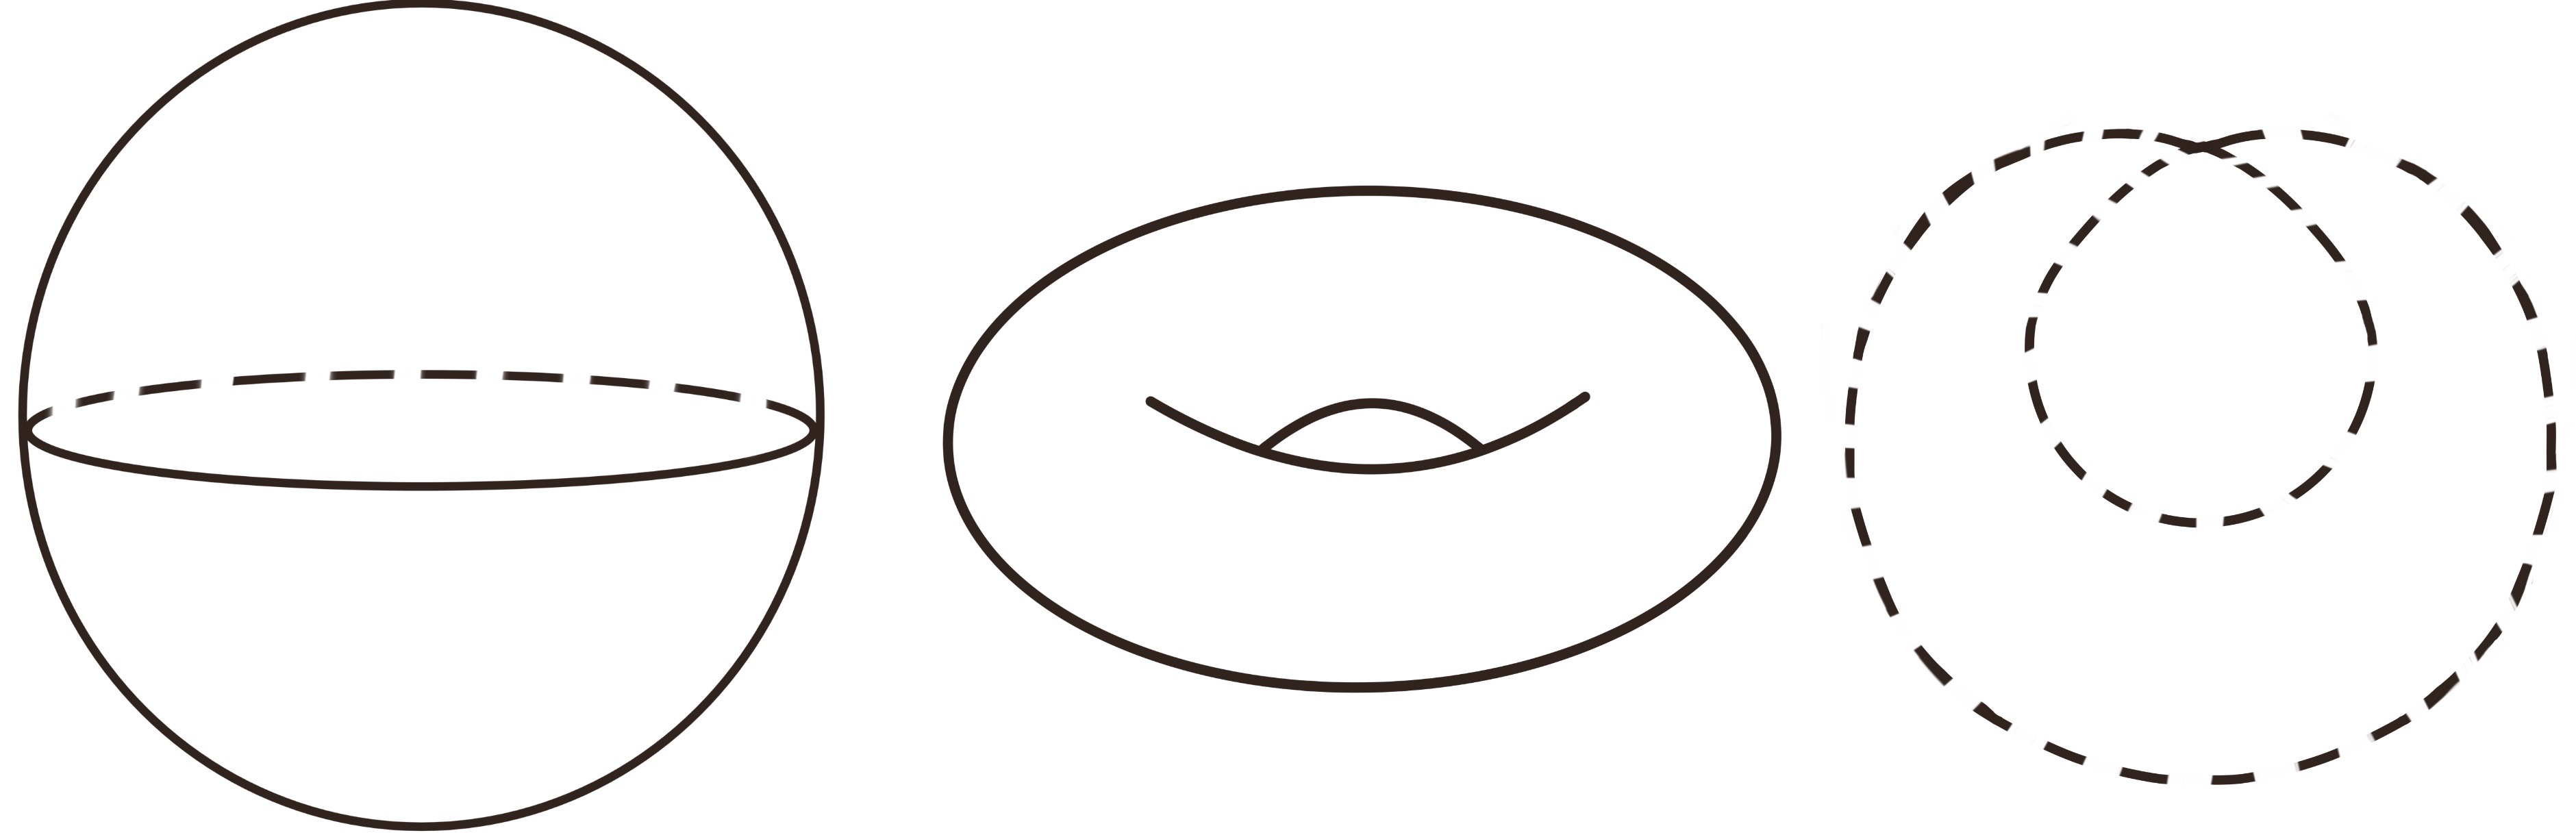
\includegraphics[width=0.5\linewidth]{imagenes/superficies.png}
	\caption{Ejemplos de superficies: Esfera, toro y banda de M\"obius}
	\label{fig:superficies sencillas}
\end{figure} 

\end{abstract}

\begin{abstract}[english]
Here goes something

\end{abstract}


\mainmatter
\chapter{Introducción}


El trabajo abarcará un estudio de las superficies topológicas y su clasificación:
\\

  
  Comenzaremos por introducir la noción de superficie de forma rigurosa. Una vez familiarizados con este concepto, tendremos como primer objetivo clasificar las superficies bajo la hipótesis de compacidad. Para ello definiremos la suma conexa y la triangulación, siendo ambas herramientas que nos facilitarán el manejo de las superficies compactas. Finalmente, enunciaremos y demostraremos el teorema de clasificación de las superficies compactas, teorema que nos garantizará que toda superficie compacta es necesariamente homeomorfa: o a una esfera; o a una \textquoteleft suma\textquoteright  finita de toros; o a una suma \textquoteleft suma\textquoteright  finita de planos proyectivos.
 \\
  
  Como segundo objetivo, estudiaremos el resultado de K\`er\`ejártó. El teorema generaliza la clasificación retirando la exigencia de compacidad. Antes de sumergirnos en el teorema, serán necesarias nuevas herramientas que nos permitan manejar las superficies no compactas. Por ello, introduciremos las nociones de finales, frontera ideal y clases de orientabilidad.
  \\
  
  Por último, examinaremos una demostración de Ian Richards \cite{ian} que  construye una superficie representante para cada clase de equivalencia topológica. Adelantamos que la construcción revela una espectacular relación entre las superficies y los subconjuntos del conjunto de Cantor.

\section{Introducci\'on a las superficies topológicas}


El concepto de superficie topológica busca generalizar la idea de \textit{superficie} en el sentido usual. Más concretamente, buscamos abarcar todo conjunto que comparta localmente las propiedades topológicas de una superficie en $\mathbb{R}^n$. 

\begin{defin}
	Diremos que un espacio topológico, $S$, es una \textbf{superficie topológica} si para todos sus puntos existe un entorno homeomorfo a $U^2 = \{x\in \mathbb{R}^2: ||x||<1 \}$. Además, a $X$ se le exige ser Hausdorff, segundo numerable y conexo. \footnote{Si retiramos la hipótesis de conexión y sustituimos $U^2$ por $U^n$, obtenemos una \textit{n-variedad} topológica. Sin embargo, en este trabajo nos limitamos al estudio de las 2-variedades conexas (superficies).}
\end{defin}

Consideremos los siguientes ejemplos sencillos de superficies topológicas:
\begin{enumerate}
	\item El conjunto $ U^2 = \{ x\in\mathbb{R}^2: |x|<1 \} $, dotado de la topología de subespacio, es trivialmente una superficie. 
	\item El cuadrado sin bordes
	\[
	C = \{(x,y)\in \mathbb{R}^2: 0 <  x < 1,\, 0 < y < 1 \}
	\]
	al ser dotado de la topología de subespacio, también es ejemplo de superficie.
	\item Dado un homeomorfismo cualquiera:
	\[
	f:S \rightarrow X
	\]
	tendremos que si $S$ es una superficie topológica, entonces $f(S)$ también lo es.
\end{enumerate}

Por otro lado, si consideramos el cuadrado con sus bordes ($\overline{C}$), el conjunto no compone un ejemplo de superficie. En este conjunto los puntos que pertenecen a las aristas no tienen entornos homeomorfos a $U^2$. Veremos que $\overline{C}$ es una \textquoteleft superficie con borde \textquoteright, concepto que estudiaremos más adelante.


\section{Orientación de superficies}
Hablar de la definición en R2.\\
Desplazamientos de una base por R2. \\
Extender la noción localmente a una superficie topológica.\\
Caminos que preservan la orientación, y caminos que la invierten (ejemplos?).\\
Superficies orientables y no orientables\\
Resultado de que los homeomorfismo preservan la orientabilidad.\\



\section{Superficies compactas}

En nuestro objetivo de acercarnos a una clasificación  completa de superficies, empezaremos por estudiar el caso de las superficies compactas. Para ello necesitaremos primero hacernos con un bagaje de ejemplos de superficies compactas elementales. Sin más preámbulo, alimentemos la curiosidad del lector con estos suculentos ejemplos:

\subsection*{La esfera}
El conjunto $ \mathbb{S}^2 = \{x\in \mathbb{R}^3: |x|=1 \} $ claramente conforma un ejemplo de superficie compacta. Alternativamente, se puede expresar la esfera como el disco $ D = \{(x,y)\in\mathbb{R}^2: |(x,y)|\leq1 \} $, realizando la identificación  \ref{esferaid} y dotando al conjunto resultante de la topología cociente.
\begin{align}\label{esferaid}
	(x,y)\equiv(x,-y),\quad\forall(x,y)\in fr(D)
\end{align}
Se puede comprobar que ambas formas de definir la esfera son homeomorfas. 

\begin{figure}[h!]
	\centering
	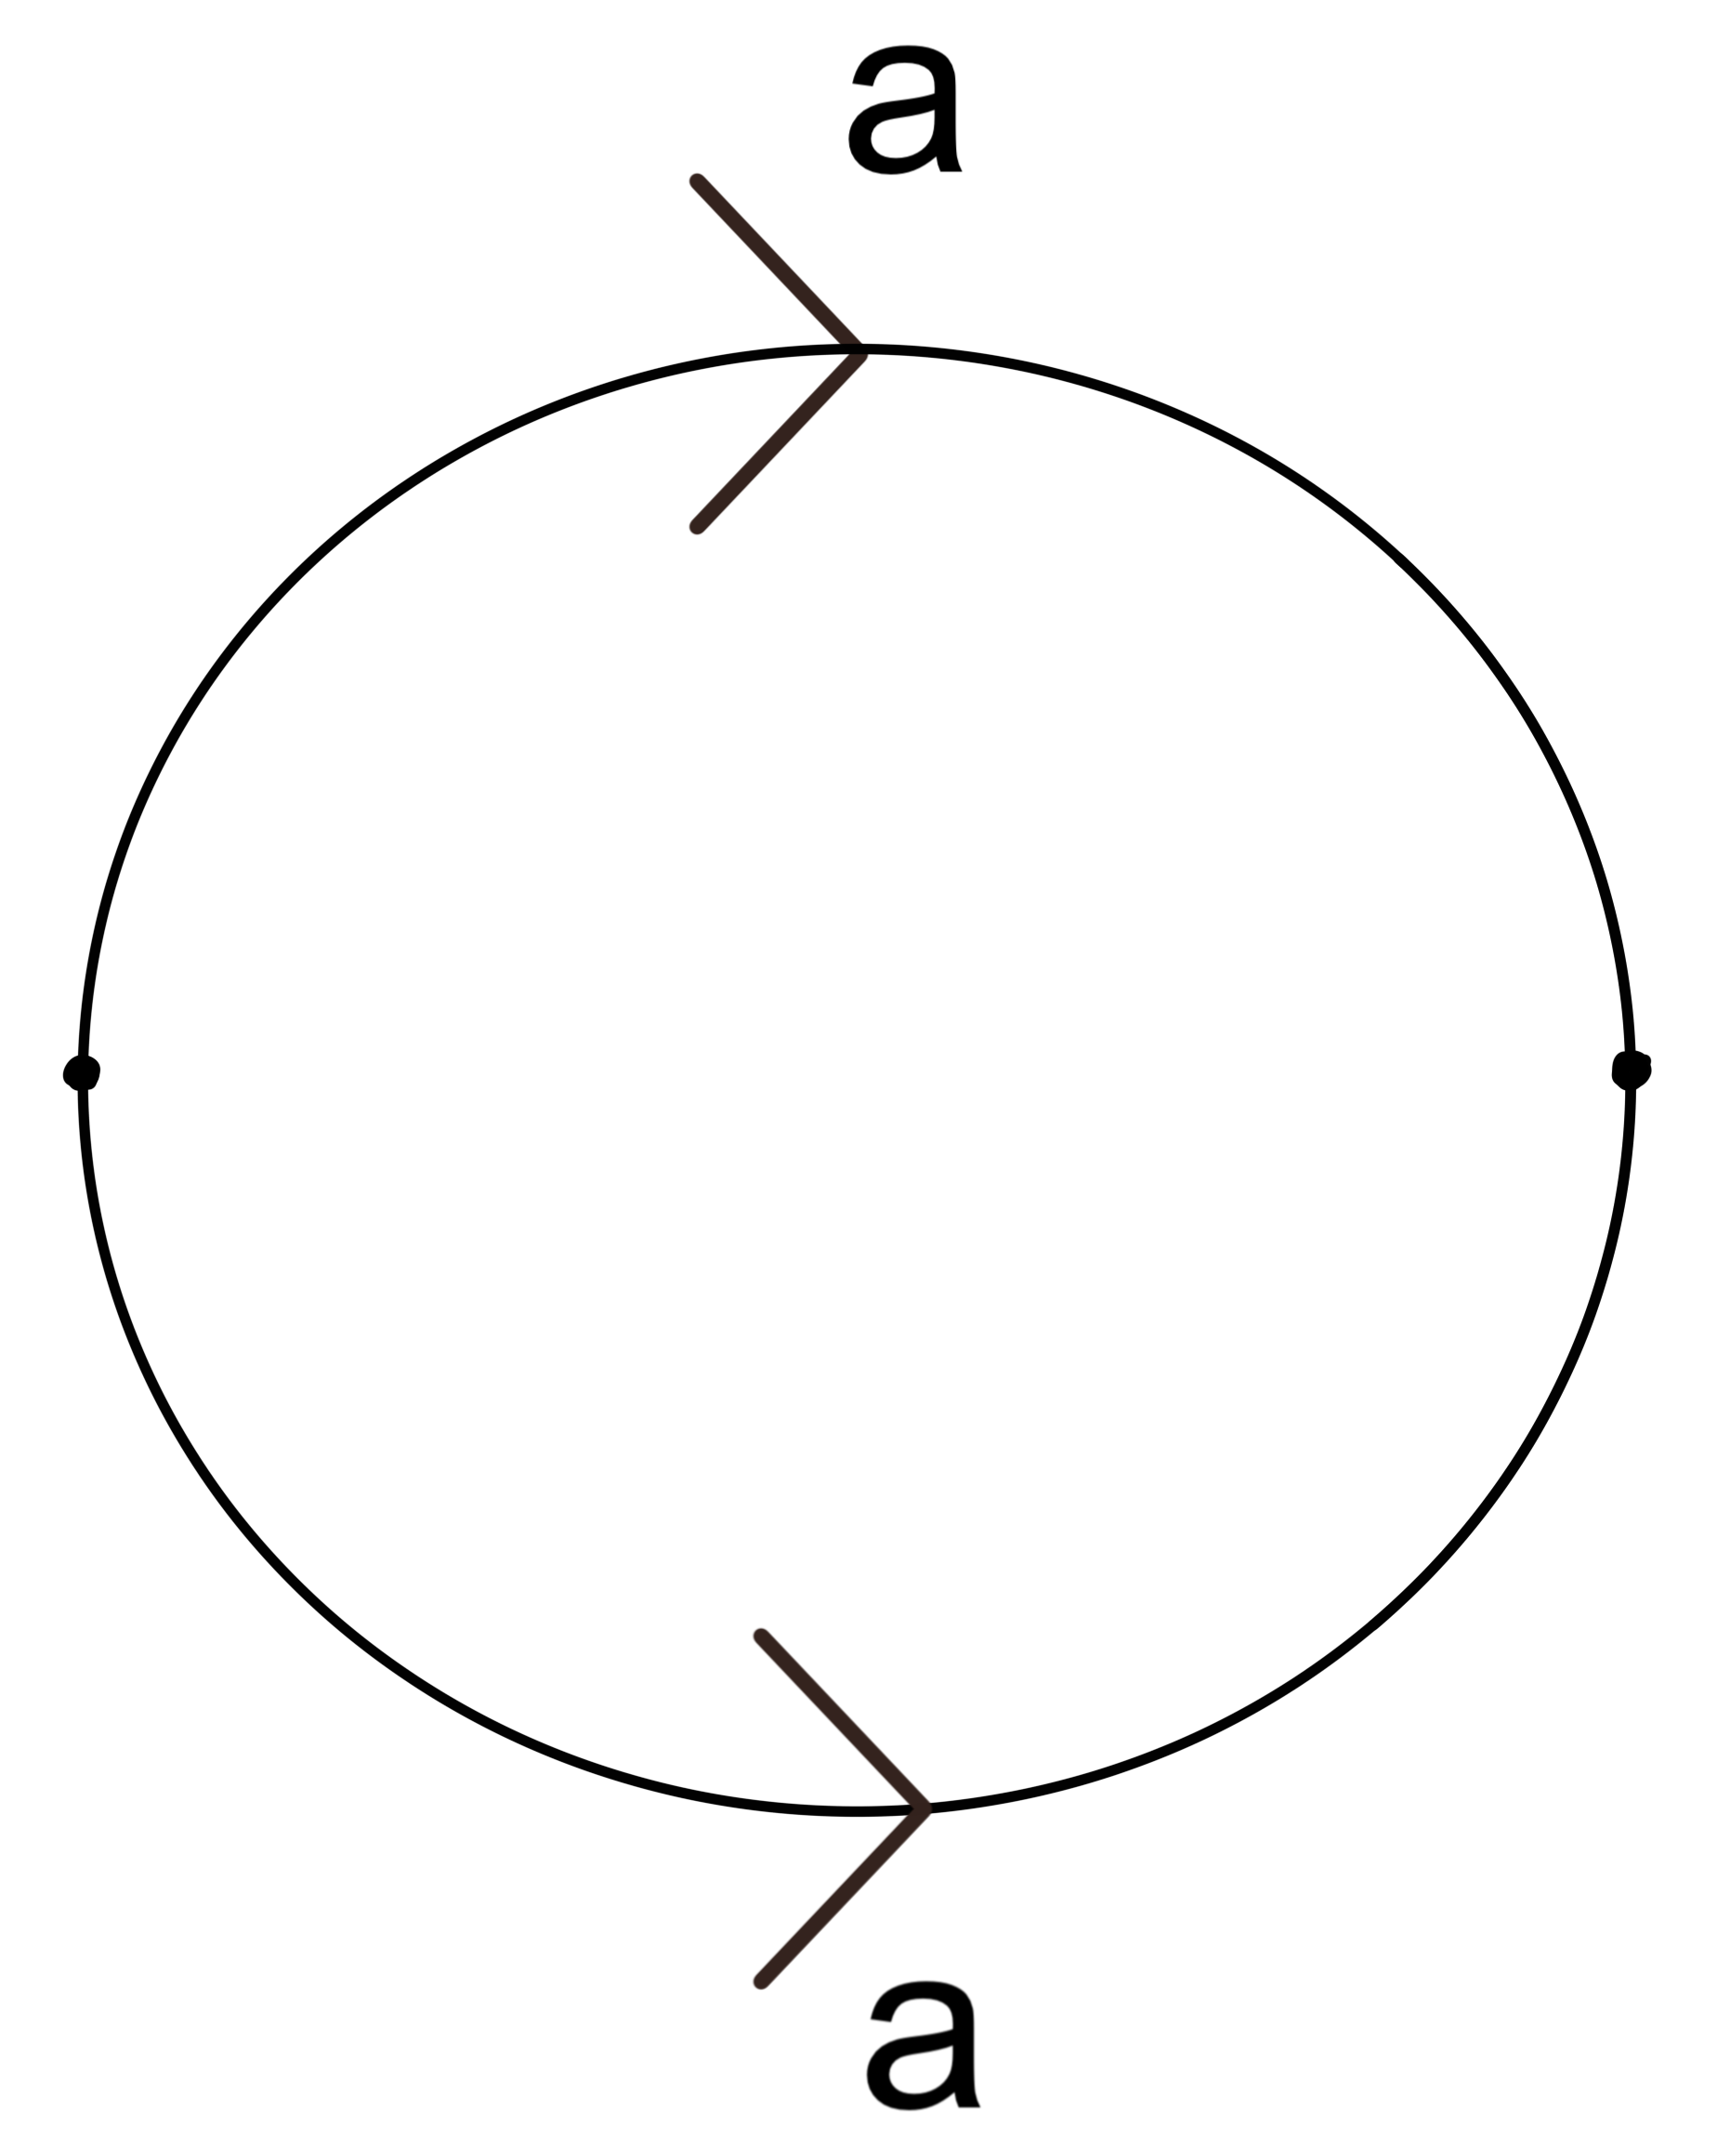
\includegraphics[width=0.2\linewidth]{imagenes/esfera_plana.png}
	\caption{Esfera como espacio cociente}
	\label{fig:esfera expresion canonica}
\end{figure} 

\subsection*{El toro}
Si se toma el cuadrado cerrado $ X = \{ (x,y) \in R^2: -1\leq x\leq 1,\quad -1\leq y \leq 1  \} $ con la topología de subespacio, el \textbf{toro}  se construye de identificar los puntos de  $ X $ según  \ref{toroid} y dotar al conjunto resultante de la topología cociente.
\begin{align}\label{toroid}
	(x,-1)\equiv(x,1) \quad x\in [-1,1]  \\
	(-1,y)\equiv(1,y) \quad y\in [-1,1] \nonumber
\end{align}

En la figura \ref{fig:toro expresion canonica} se representa gráficamente el toro. Las aristas con el mismo símbolo indican aristas a identificar en el sentido indicado por las flechas.

\begin{figure}[h!]
	\centering
	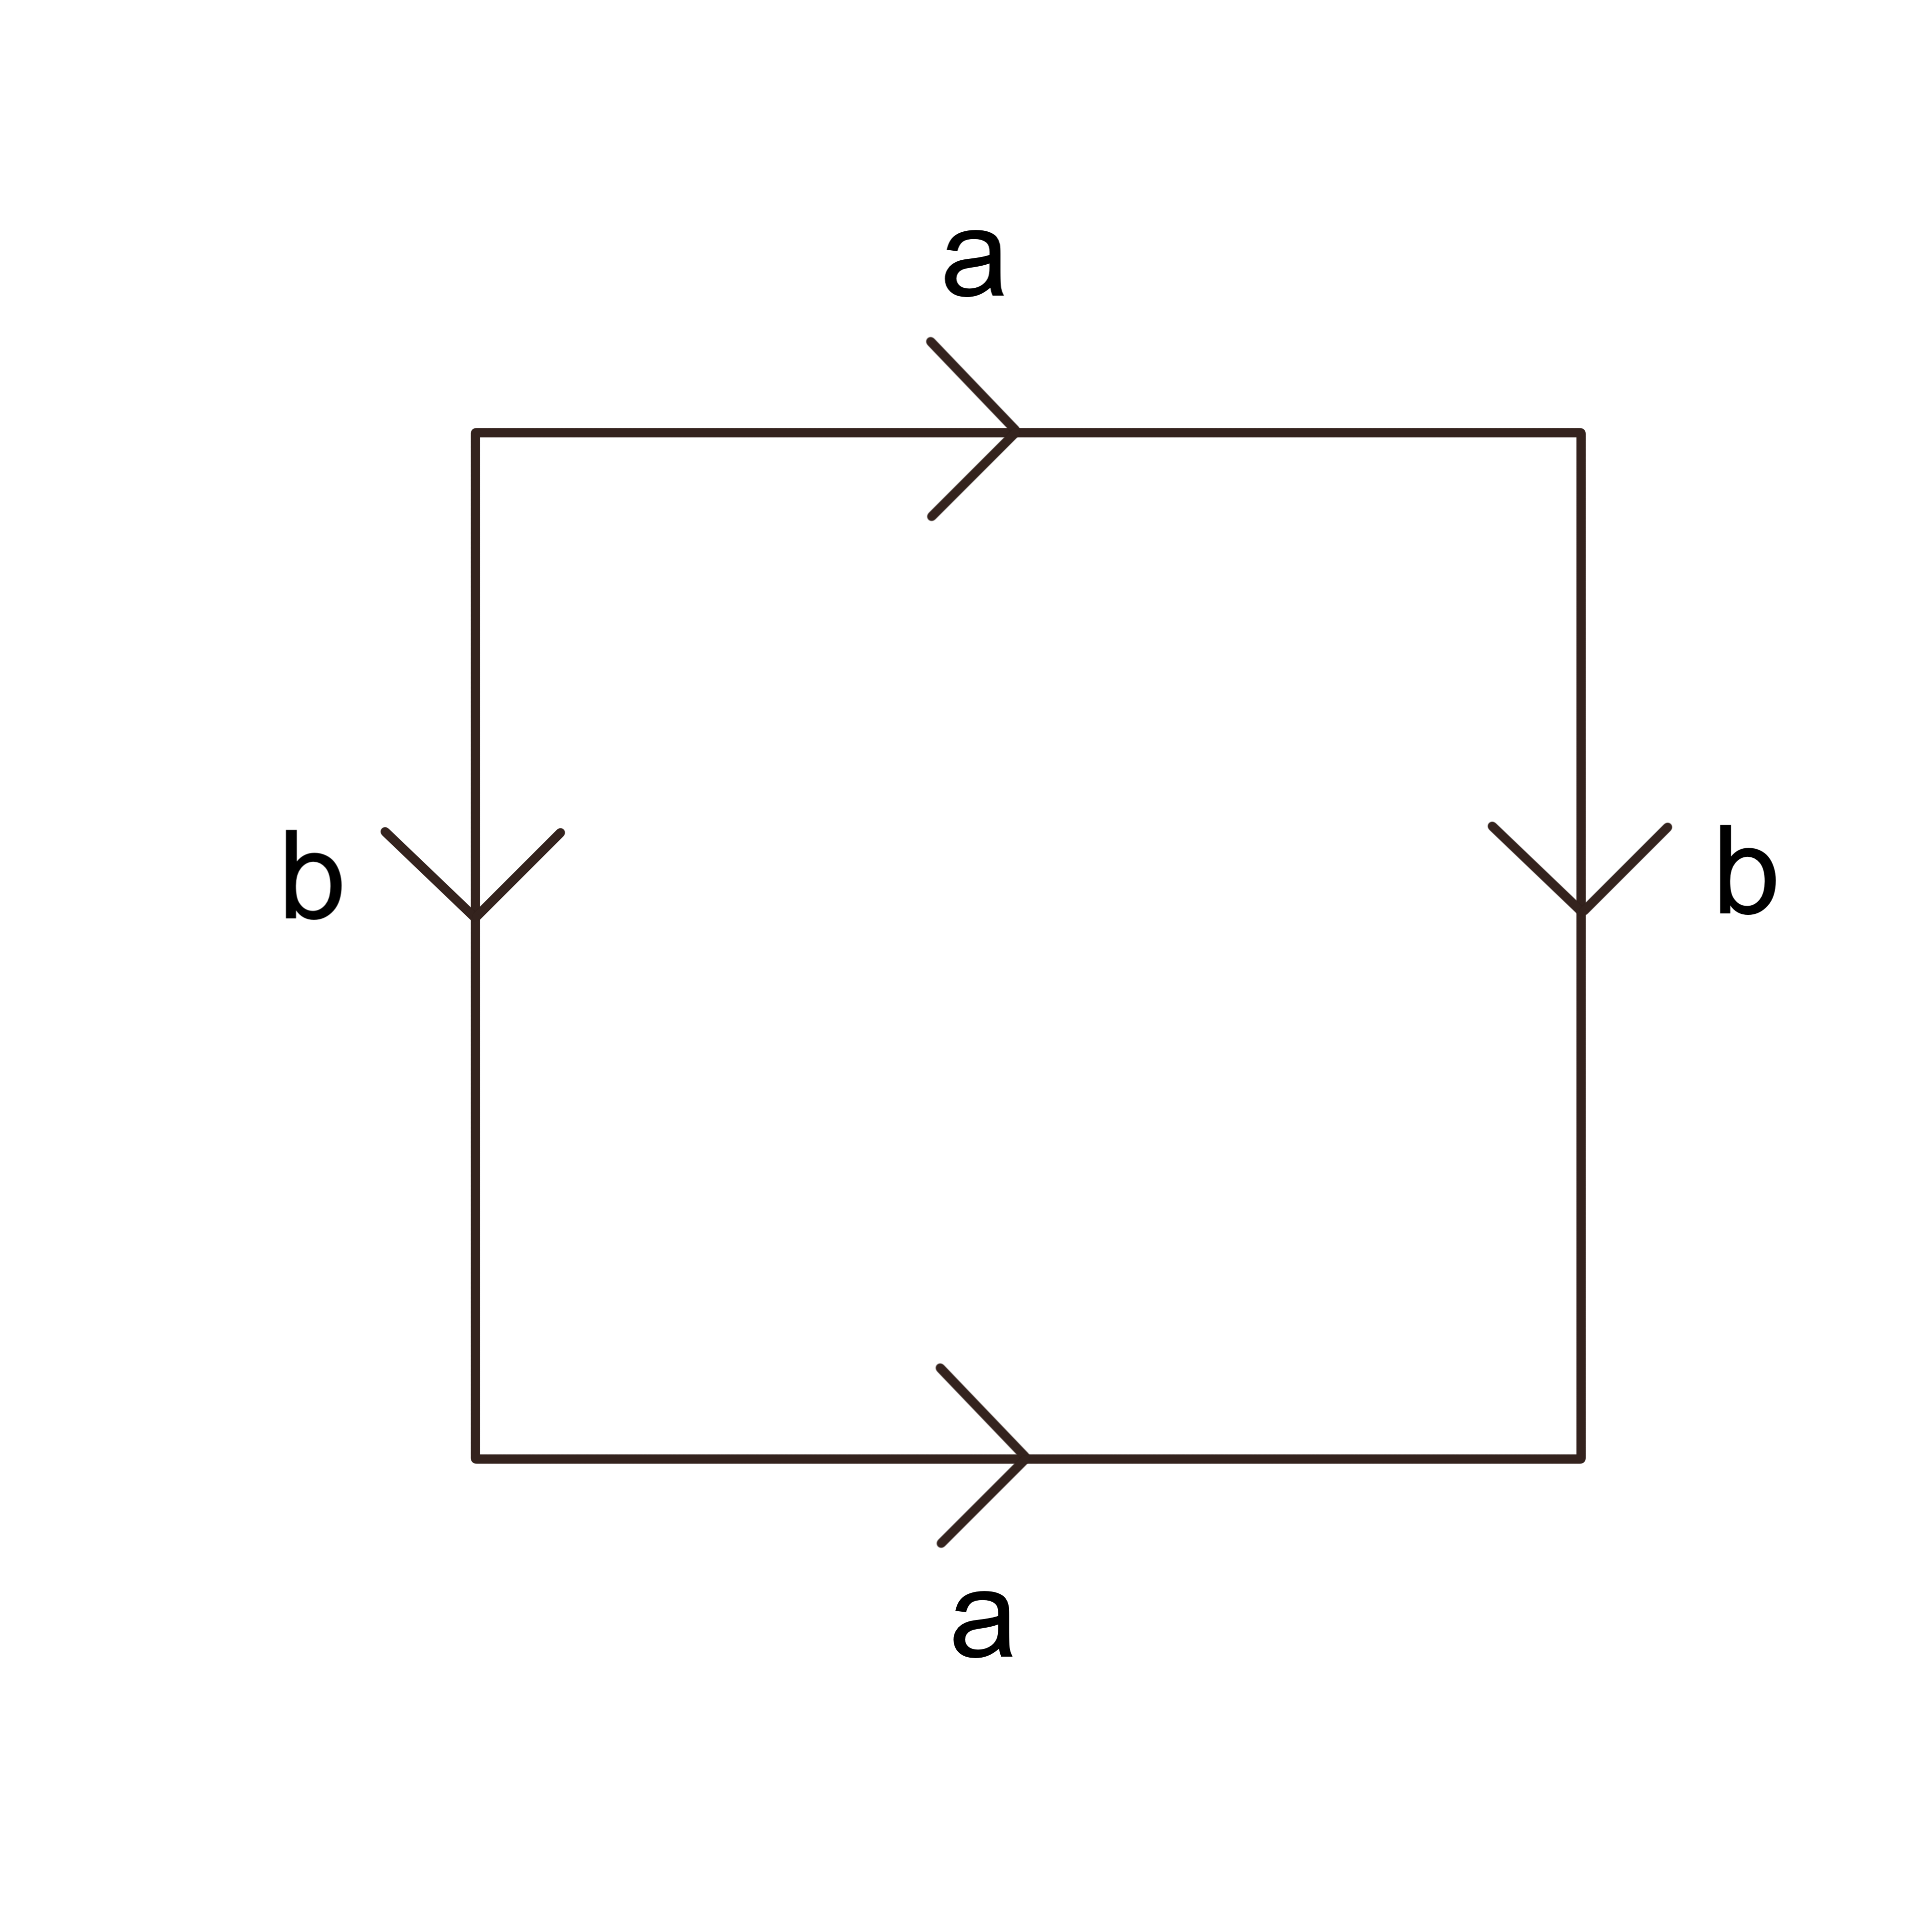
\includegraphics[width=0.3\linewidth]{imagenes/toroplano.png}
	\caption{Toro como espacio cociente}
	\label{fig:toro expresion canonica}
\end{figure} 


\subsection*{El plano proyectivo}
Por su parte, el \textbf{plano proyectivo} corresponde al disco $ D = \{x\in\mathbb{R}^2: ||x||\leq1 \} $ en el cual se identifican los puntos antipodales de la frontera. Se ilustra esta identificación en la figura \ref{fig:planoproyectivo expresión canónica}.

\begin{figure}[h!]
	\centering
	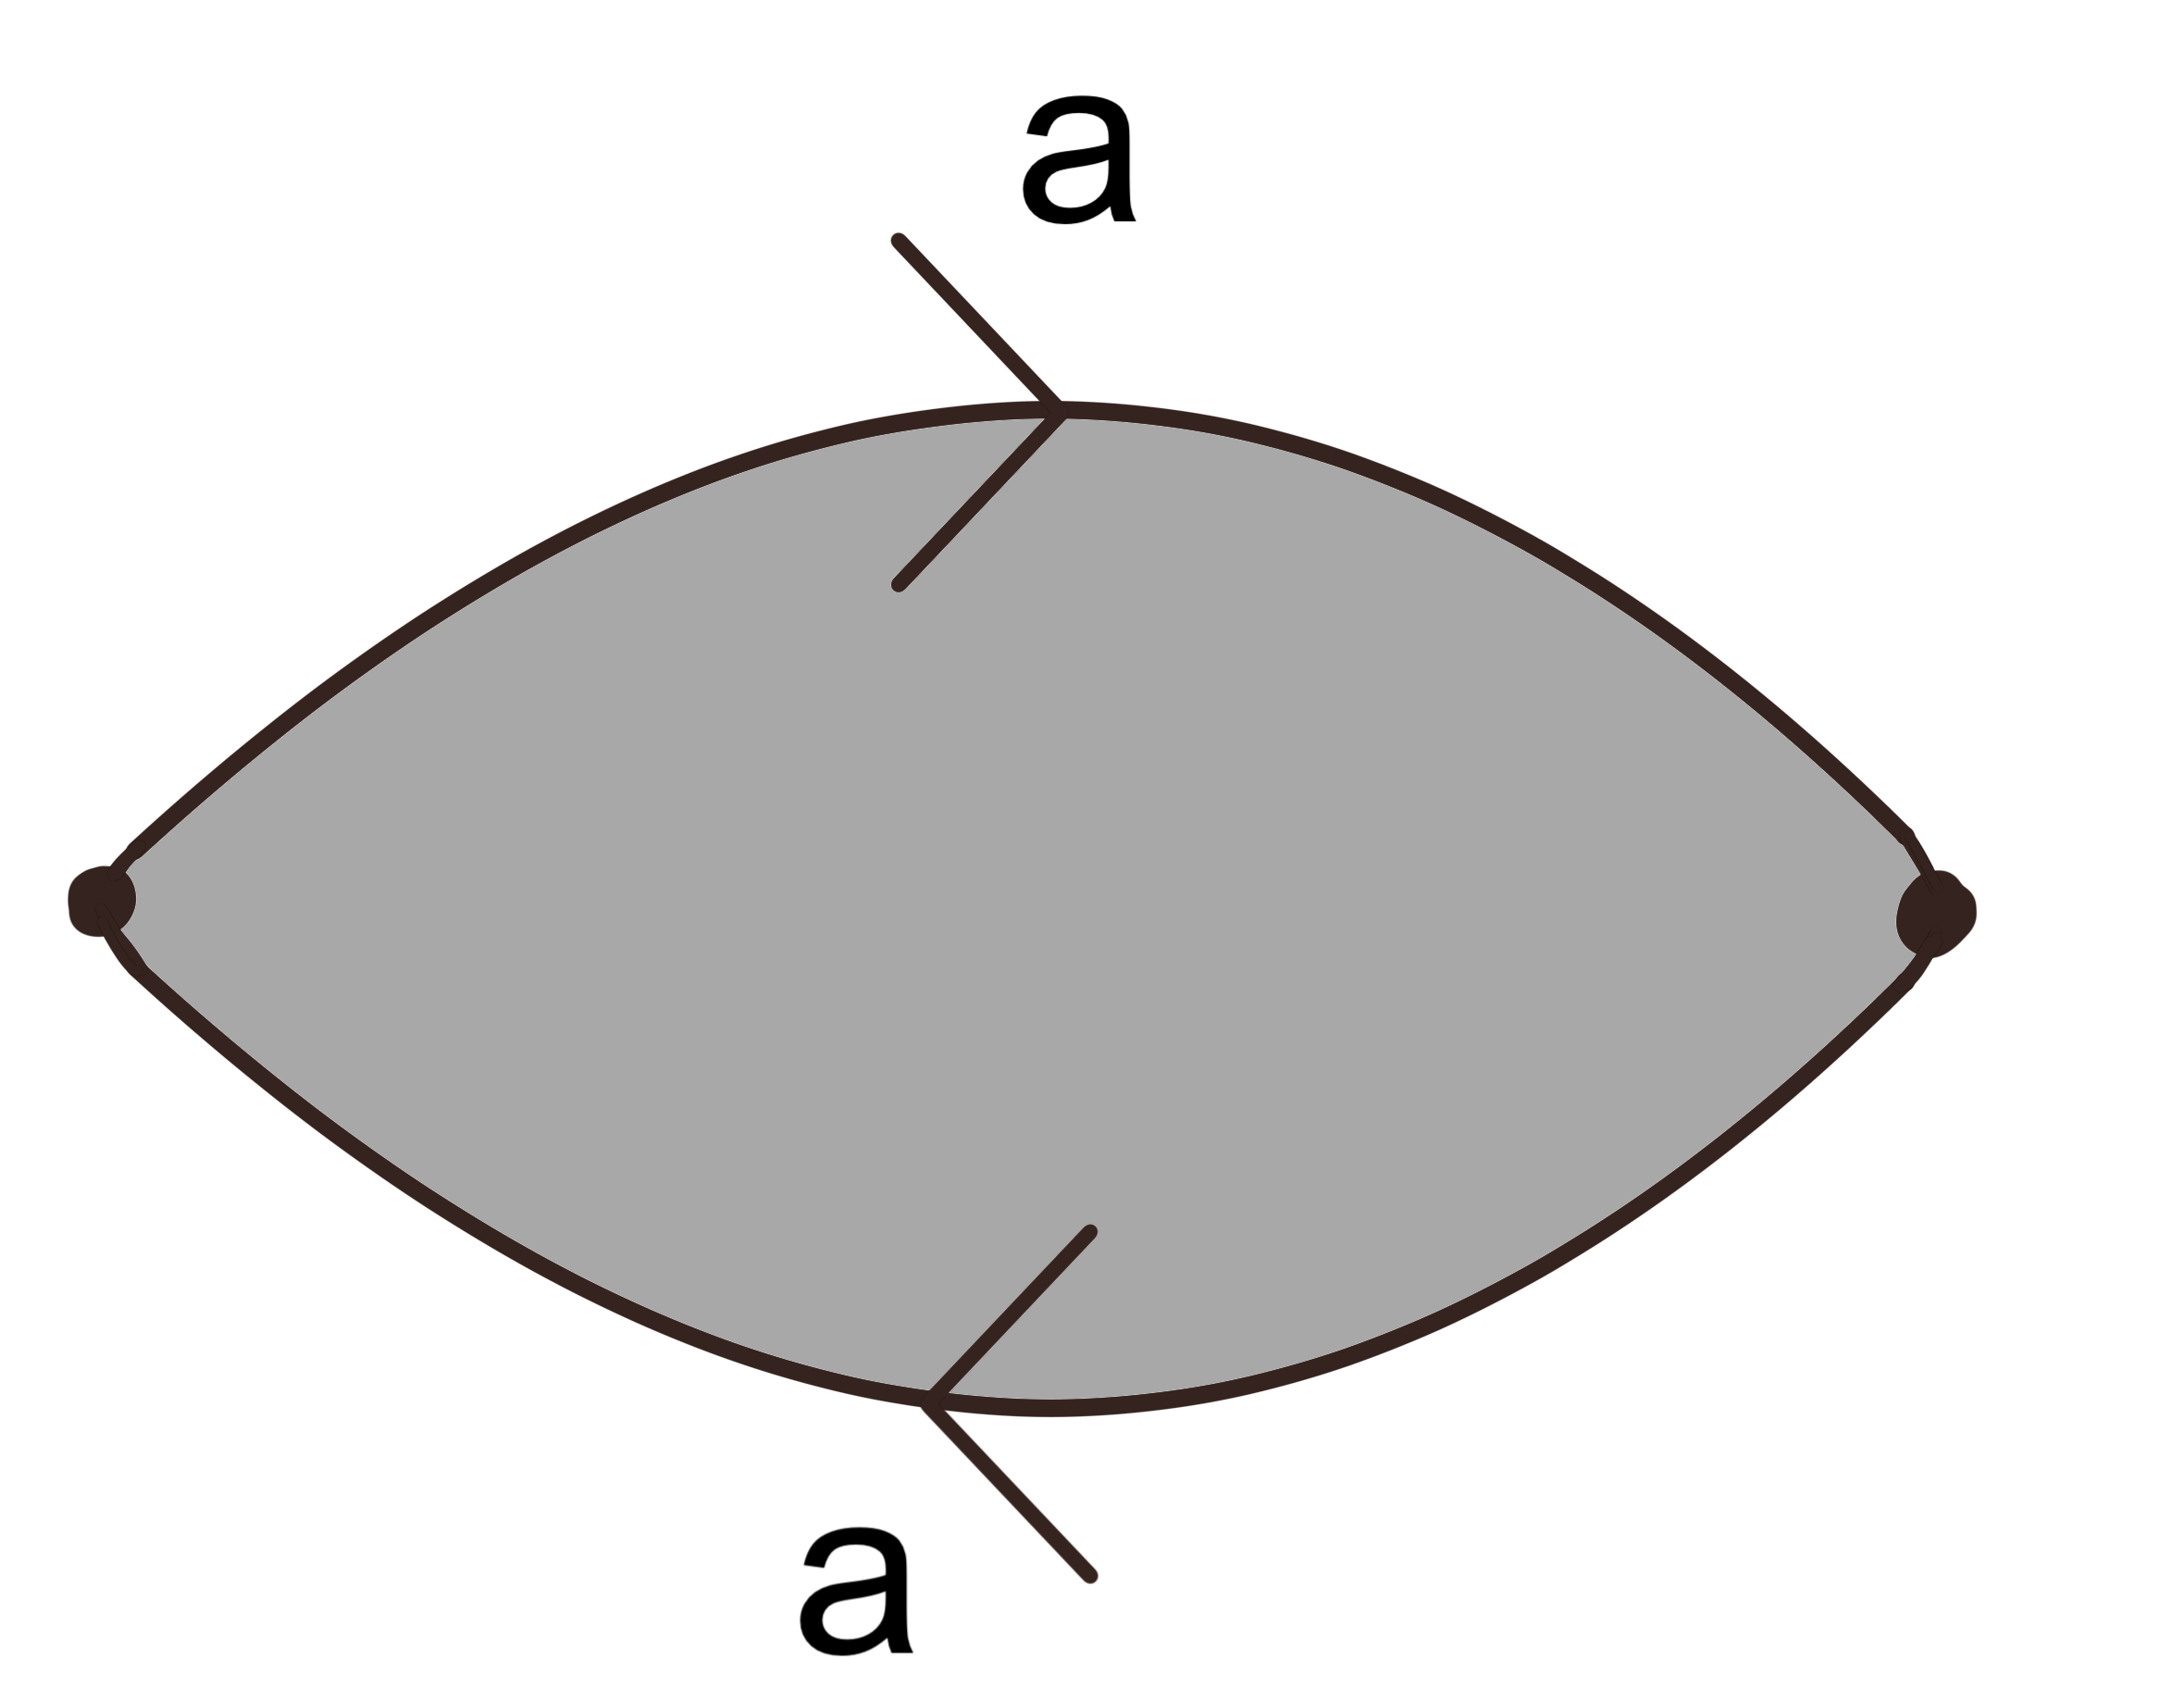
\includegraphics[width=0.3\linewidth]{imagenes/planop_plano.png}
	\caption{Plano proyectivo como espacio cociente}
	\label{fig:planoproyectivo expresión canónica}
\end{figure} 

De los tres ejemplos de superficies compactas dadas hasta ahora, este es el único de una superficie no orientable. 
\\

Después de haber visto los ejemplos, es razonable cuestionarse si los espacios cocientes que tratamos en ellos son realmente conjuntos compactos. El siguiente lema nos demuestra que, en efecto, las superficies obtenidas son compactas.

\begin{lema}\label{lema:compacidadDePoligonos}
	Sea $X$ un espacio topológico e $Y$  un espacio cociente que resulta de identificar puntos en $X$. Entonces:
	\begin{align*}
	\text{$X$ compacto}\Rightarrow\text{$Y$ compacto}
	\end{align*}
\end{lema}
\begin{proof}
	Sea $f:X\longrightarrow Y$ la función cociente que asocia a cada punto su clase de equivalencia; $f$ es claramente sobreyectiva y, por ser cociente, es continua.\\
	Siendo $X$ compacto tenemos entonces que $f(X)=Y$ también lo es.
\end{proof}
En nuestros ejemplos todas las superficies vienen de identificar puntos en conjuntos compactos. Se sigue entonces del lema que las superficies son a su vez compactas.

\subsection*{Expresión canónica}

Las figuras \ref{fig:esfera expresion canonica}, \ref{fig:toro expresion canonica} e \ref{fig:planoproyectivo expresión canónica}, de cada ejemplo respectivamente, sugieren una forma visual de definir superficies compactas: formamos un polígono con un número par de lados e identificamos sus aristas a pares. 

Más aún, se puede definir una notación con la que referirnos a estos polígonos: \\
Partiendo de cualquier vértice recorremos la figura en el sentido de las agujas del reloj, se anotan los símbolos según se recorre la respectiva arista y se agrega el exponente 1 o -1, según si la flecha va en el mismo sentido del recorrido o en sentido contrario.

Con esta notación: nos referimos  a la esfera (figura \ref{fig:esfera expresion canonica}) como $ aa^{-1} $; al toro (figura \ref{fig:toro expresion canonica})  como $ aba^{-1}b^{-1} $; y al plano proyectivo (figura \ref{fig:planoproyectivo expresión canónica}) como $ aa $. Llamaremos \textbf{expresión canónica} a estas formas de referirnos a la esfera, al toro y al plano proyectivo, respectivamente.
\\

La notación sugerida facilita enormemente la definición de nuevas superficies. Utilicemos esta herramienta para introducir un último ejemplo de superficie compacta:


\subsection*{Botella de \textit{Klein}}
	La \textbf{botella de \textit{Klein}} es la superficie que corresponde con la expresión $ aba^{-1}b $.

\begin{figure}[h!]
	\centering
	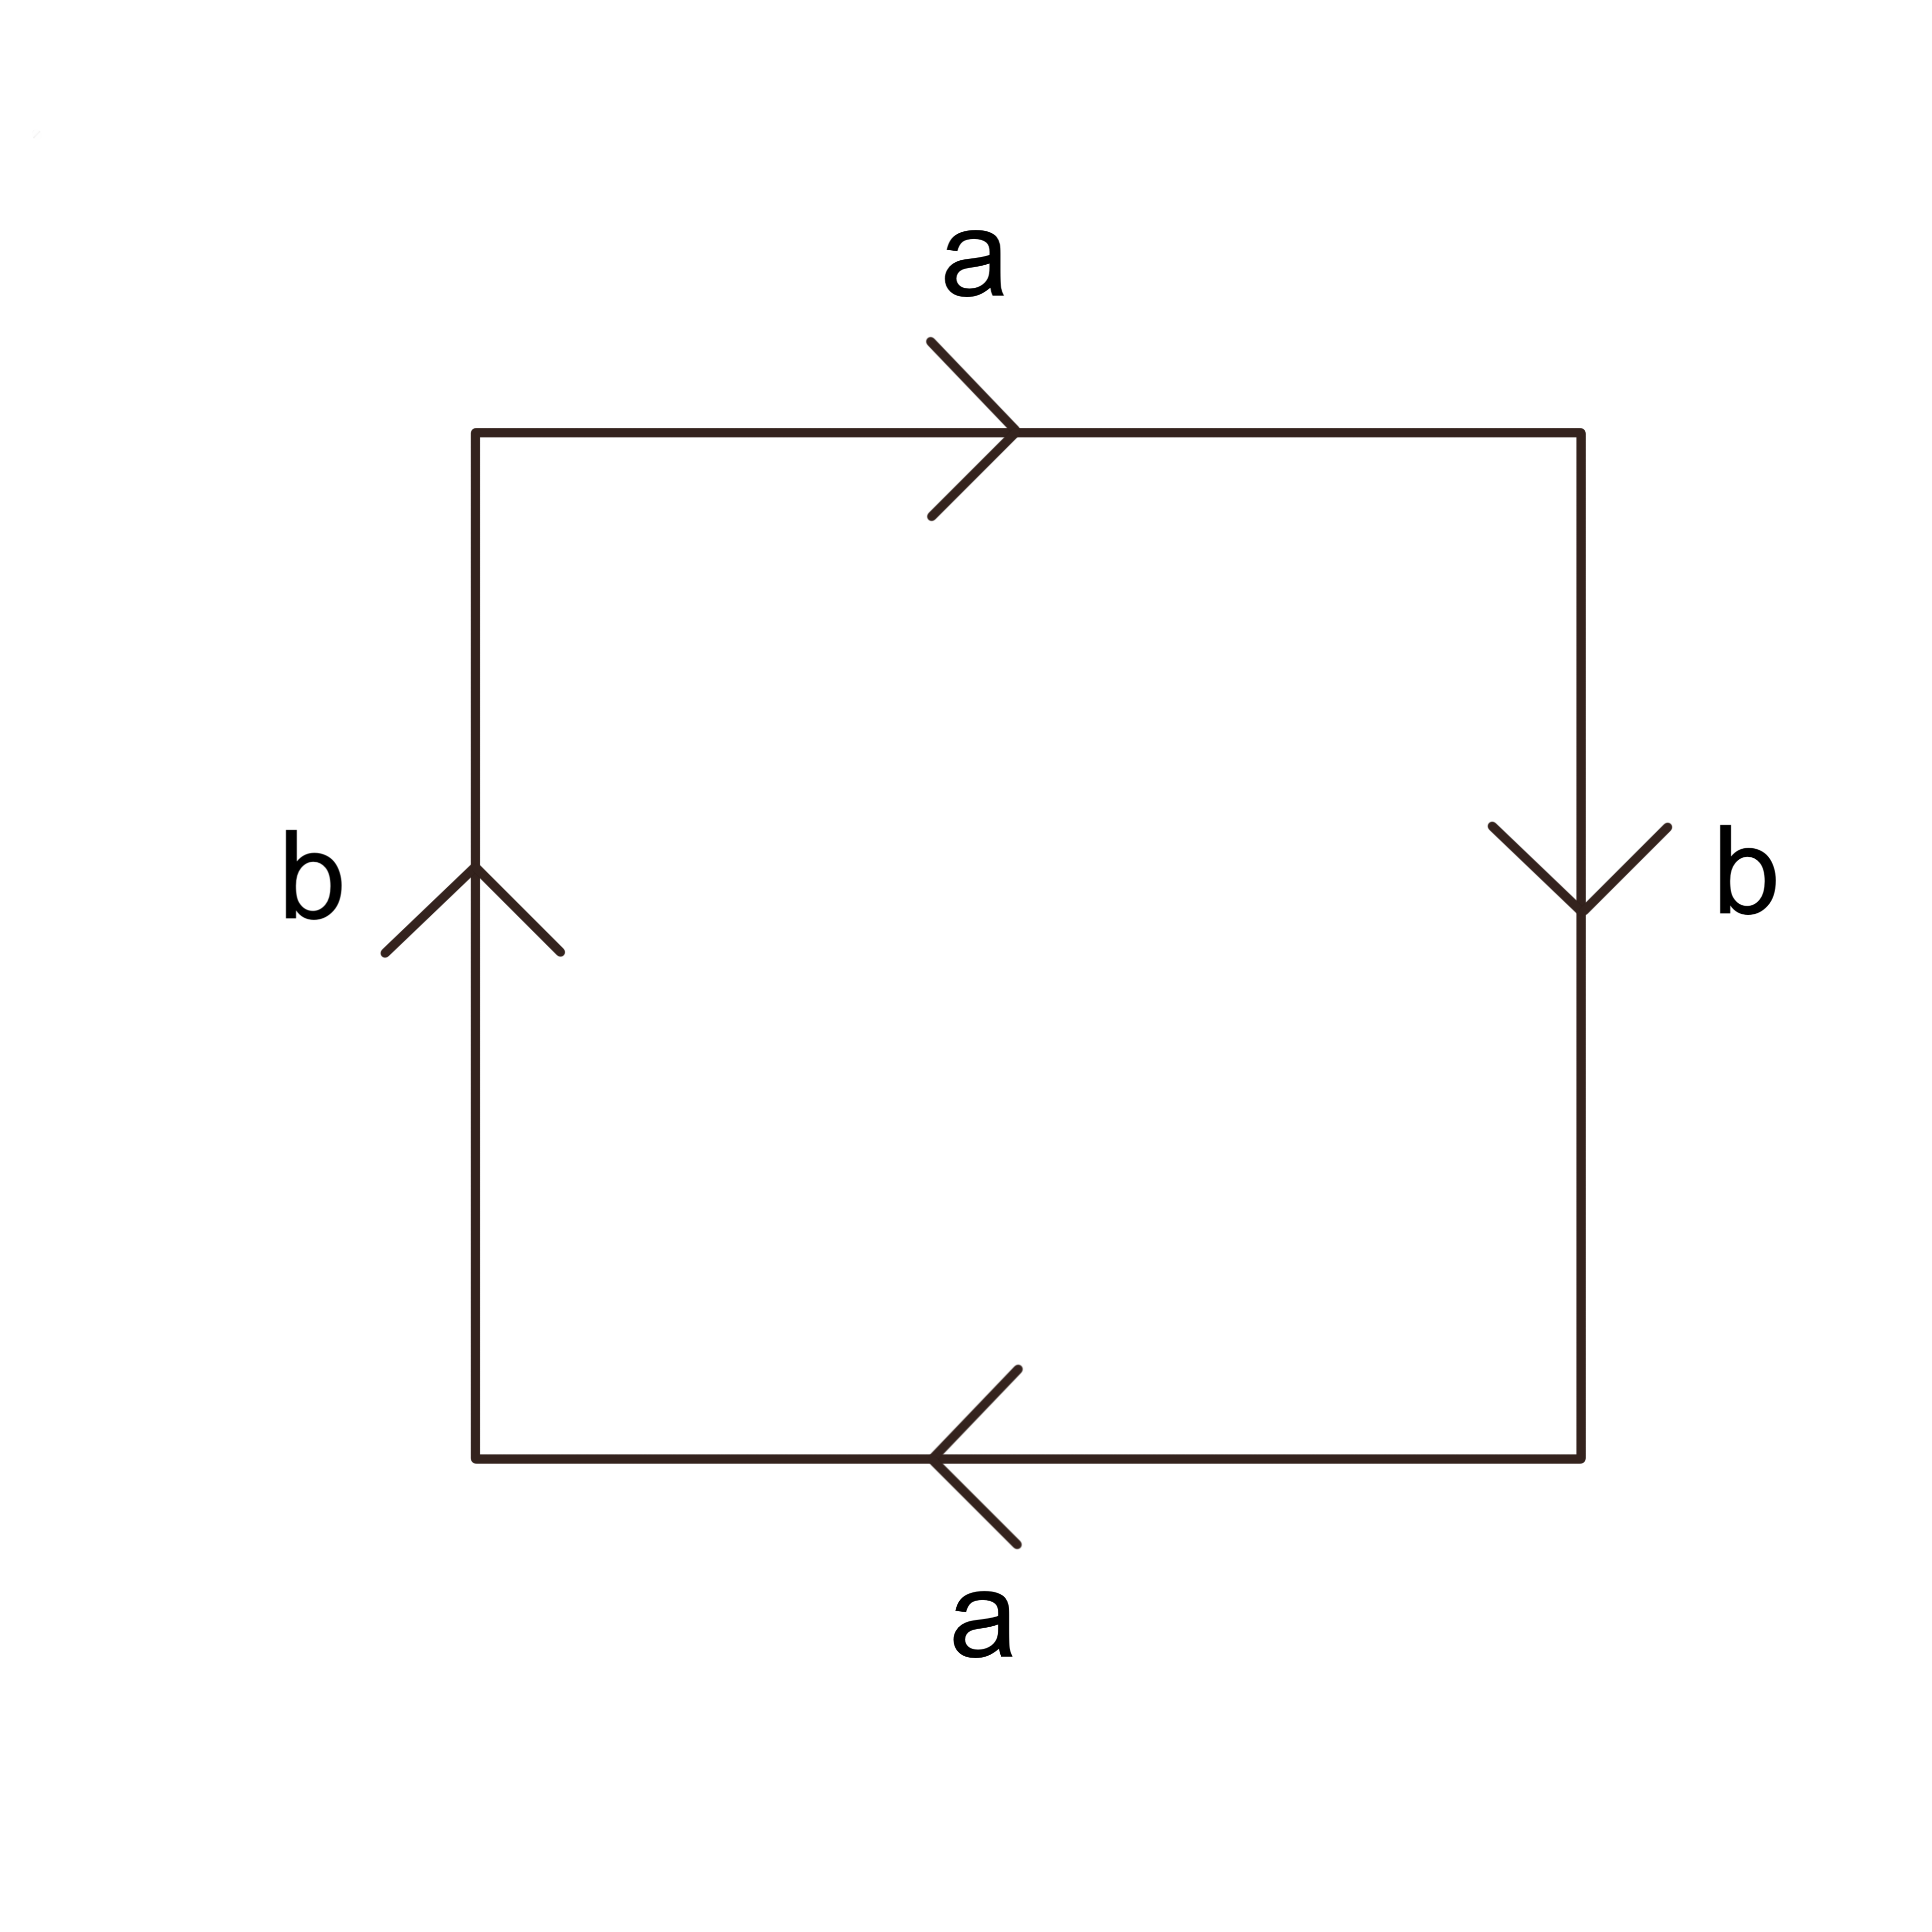
\includegraphics[width=0.3\linewidth]{imagenes/klein.png}
	\caption{Botella de Klein}
	\label{fig:botelladeklein expresion canónica}
\end{figure} 




\section{Suma conexa}

La suma conexa es un operador entre superficies. La idea será ir \textquoteleft sumando \textquoteright superficies compactas para generar nuevas. De hecho, si se me permite el \textit{spoiler}, utilizaremos este operador en toros y planos proyectivos para construir superficies homeomorfas a \textbf{cualquier} otra superficie compacta.\\
Procedamos a definir matemáticamente el operador:

\begin{defin}\label{defin:sumaconexa}
	Dadas dos superfices $S_1$ y $S_2$, se define la \textbf{suma conexa} de ambas ($S_1\#S_2$) como la superficie generada al recortar un disco de cada superficie y pegarlas a través del borde de los discos retirados. Más formalmente:
	\begin{enumerate}
		\item 
		Para cada $S_i$, tomamos un subconjunto $D_i\subset S_i$ homeomorfo al disco cerrado $E^2=\{x\in\mathbb{R}^2: ||x||\leq 1\}$. Llamamos $S'_i$ al complementario del interior de $D_i$.
		\item 
		Tomamos un homeomorfismo $\psi:D_1\longrightarrow D_2$
		\item 
		Definimos entonces $S_1\#S_2$ como $S'_1\cup S'_2$ dotado de la topología cociente que resulta de la identificación:
		\[
		x \equiv  \psi(x), \quad \forall x \in D_1
		\] 
	\end{enumerate}
	Habría que comprobar que la suma conexa está bien definida y resulta en una nueva superficie. Este aspecto lo abordamos en lema \ref{lema:sumaconexa}.
\end{defin}


\subsection*{Ejemplos}
Utilizando la notación introducida hasta el momento presentamos algunos ejemplos de sumas conexas:
\\

\noindent \textbf{Suma conexa de toros}
\\
Sean $ T_1 $ y $ T_2 $ dos toros disjuntos, estudiemos $ S=T_1\, \# \, T_2 $. Nos ayudamos de la figura \ref{fig:suma conexa de toros planos} para ilustrar el proceso:\\
Primero, retiramos de cada toro el disco con frontera $c_i$, como vemos en la primera imagen. Nótese que podemos expresarlo como la segunda imagen porque todos los vértices del polígono están identificados. Finalmente, identificamos los bordes $ c_1 $ y $ c_2 $, obteniendo el octágono que representa  $ S $, donde, de nuevo, todos los vértices representan el mismo punto.


\begin{figure}[h!]
	\centering
	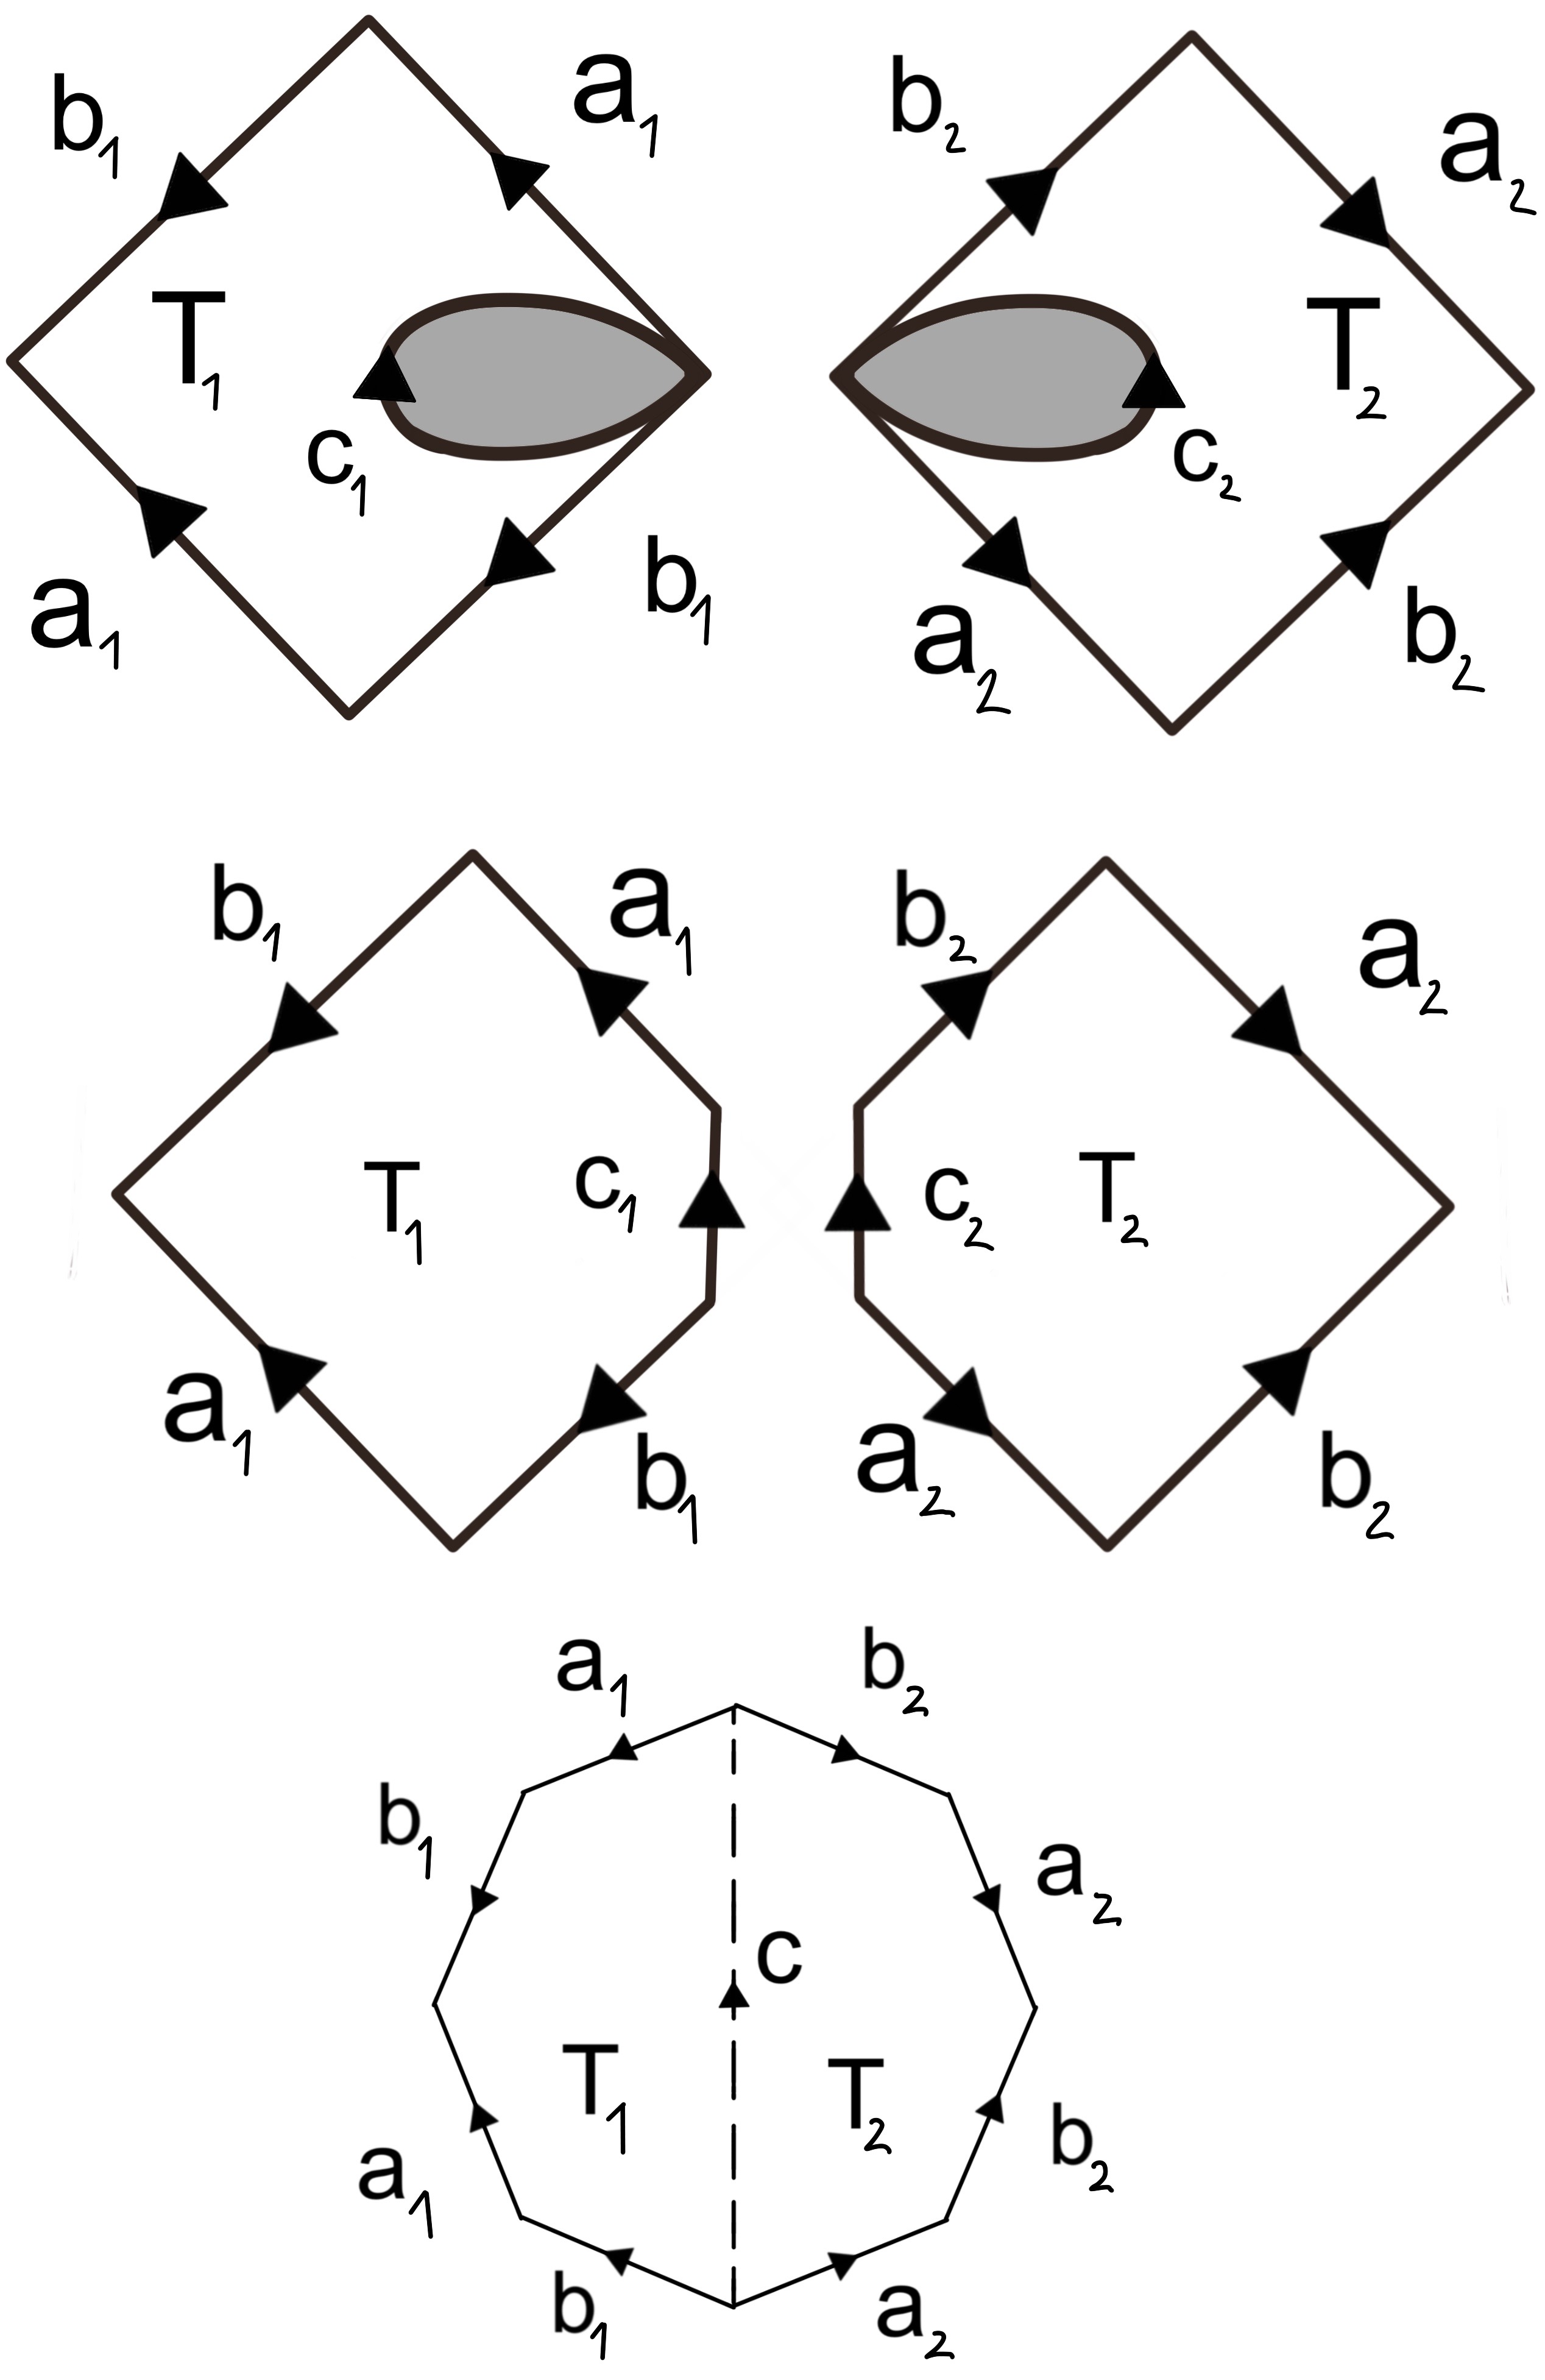
\includegraphics[width=0.4\linewidth]{imagenes/sumaconexa_toros.png}
	\caption{Suma conexa de dos toros}
	\label{fig:suma conexa de toros planos}
\end{figure} 

Utilizando la notación para expresiones canónicas, de la figura \ref{fig:suma conexa de toros planos} se deduce que  $ S $ se puede expresar como $ a_1 b_1 a_1^{-1}b_1^{-1}a_2 b_2 a_2^{-1} b_2^{-1}  $. 


\begin{figure}[h!]
	\centering
	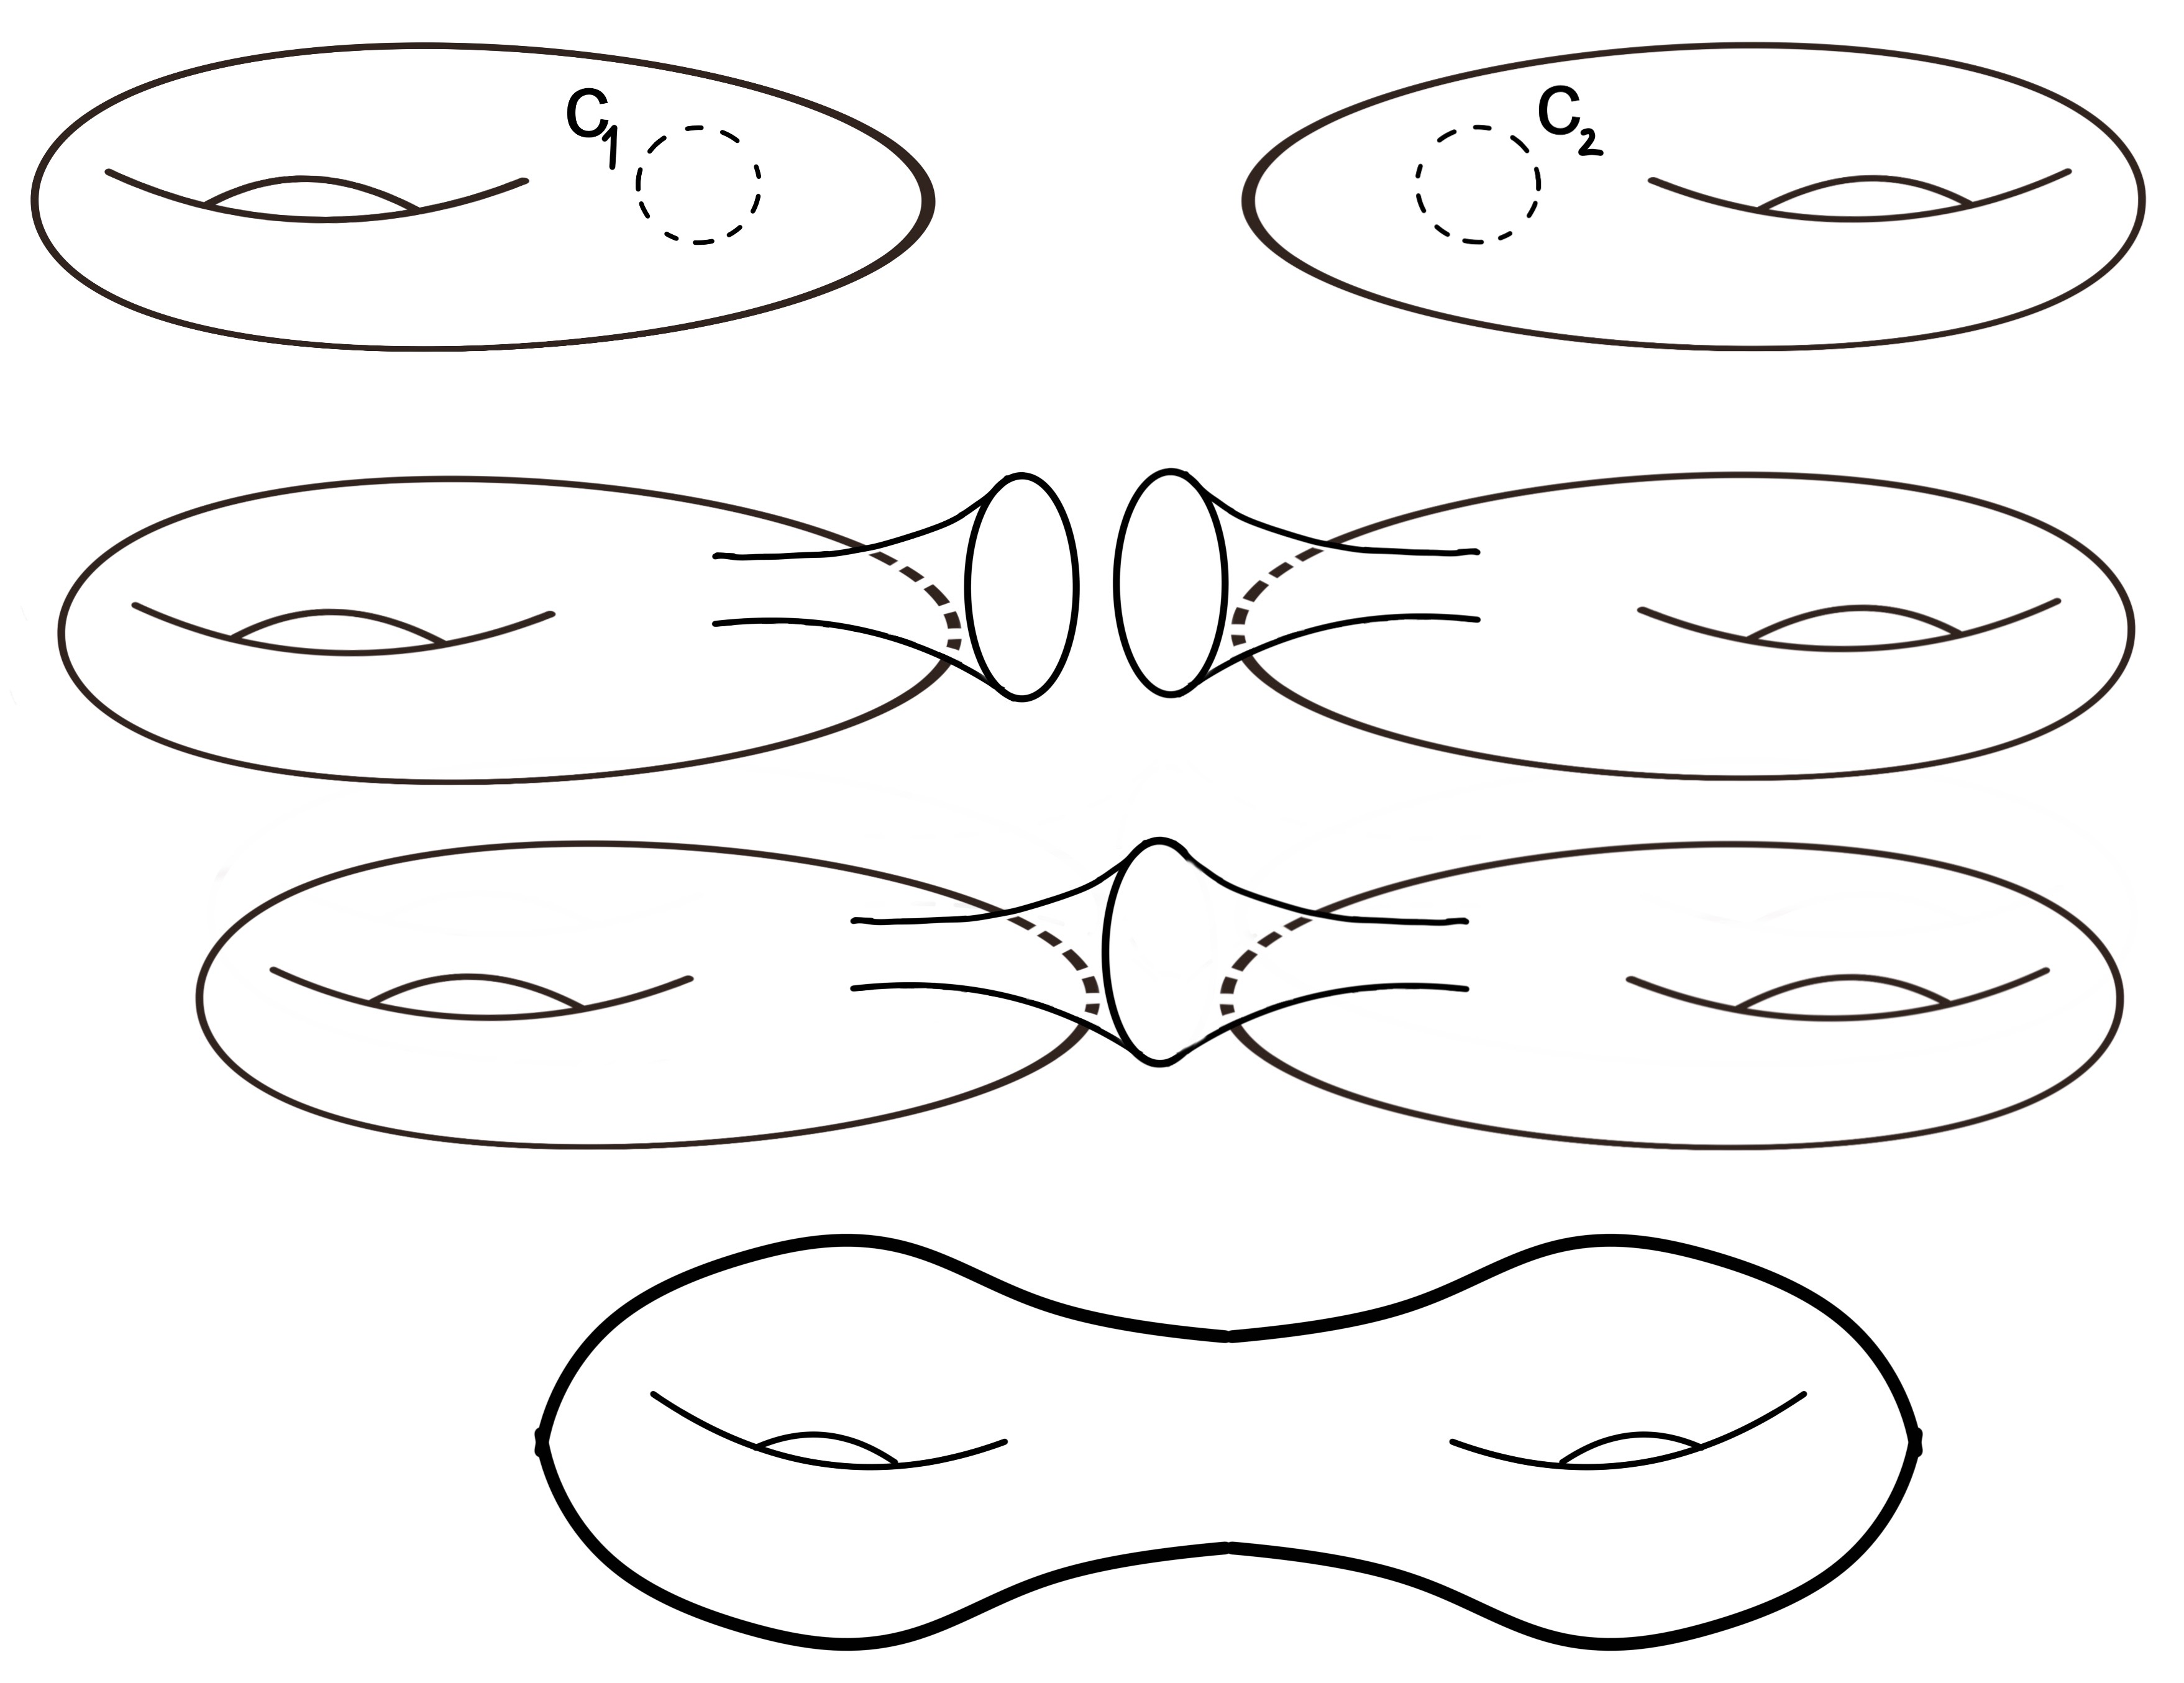
\includegraphics[width=0.4\linewidth]{imagenes/sumaconexa_toros_R3.png}
	\caption{Suma conexa de dos toros como subvariedades de $ \mathbb{R}^3 $}
	\label{fig:suma conexa de toros en R3}
\end{figure} 

\noindent \textbf{Suma conexa de planos proyectivos}
\\
Podemos seguir un mecanismo parecido al anterior para realizar la suma conexa de dos planos proyectivos. En la figura \ref{fig:suma conexa de planos p} ilustramos la misma construcción para dos planos proyectivos. La expresión canónica de la superficie resultante es $ a_1a_1a_2a_2 $.

\begin{figure}[h!]
	\centering
	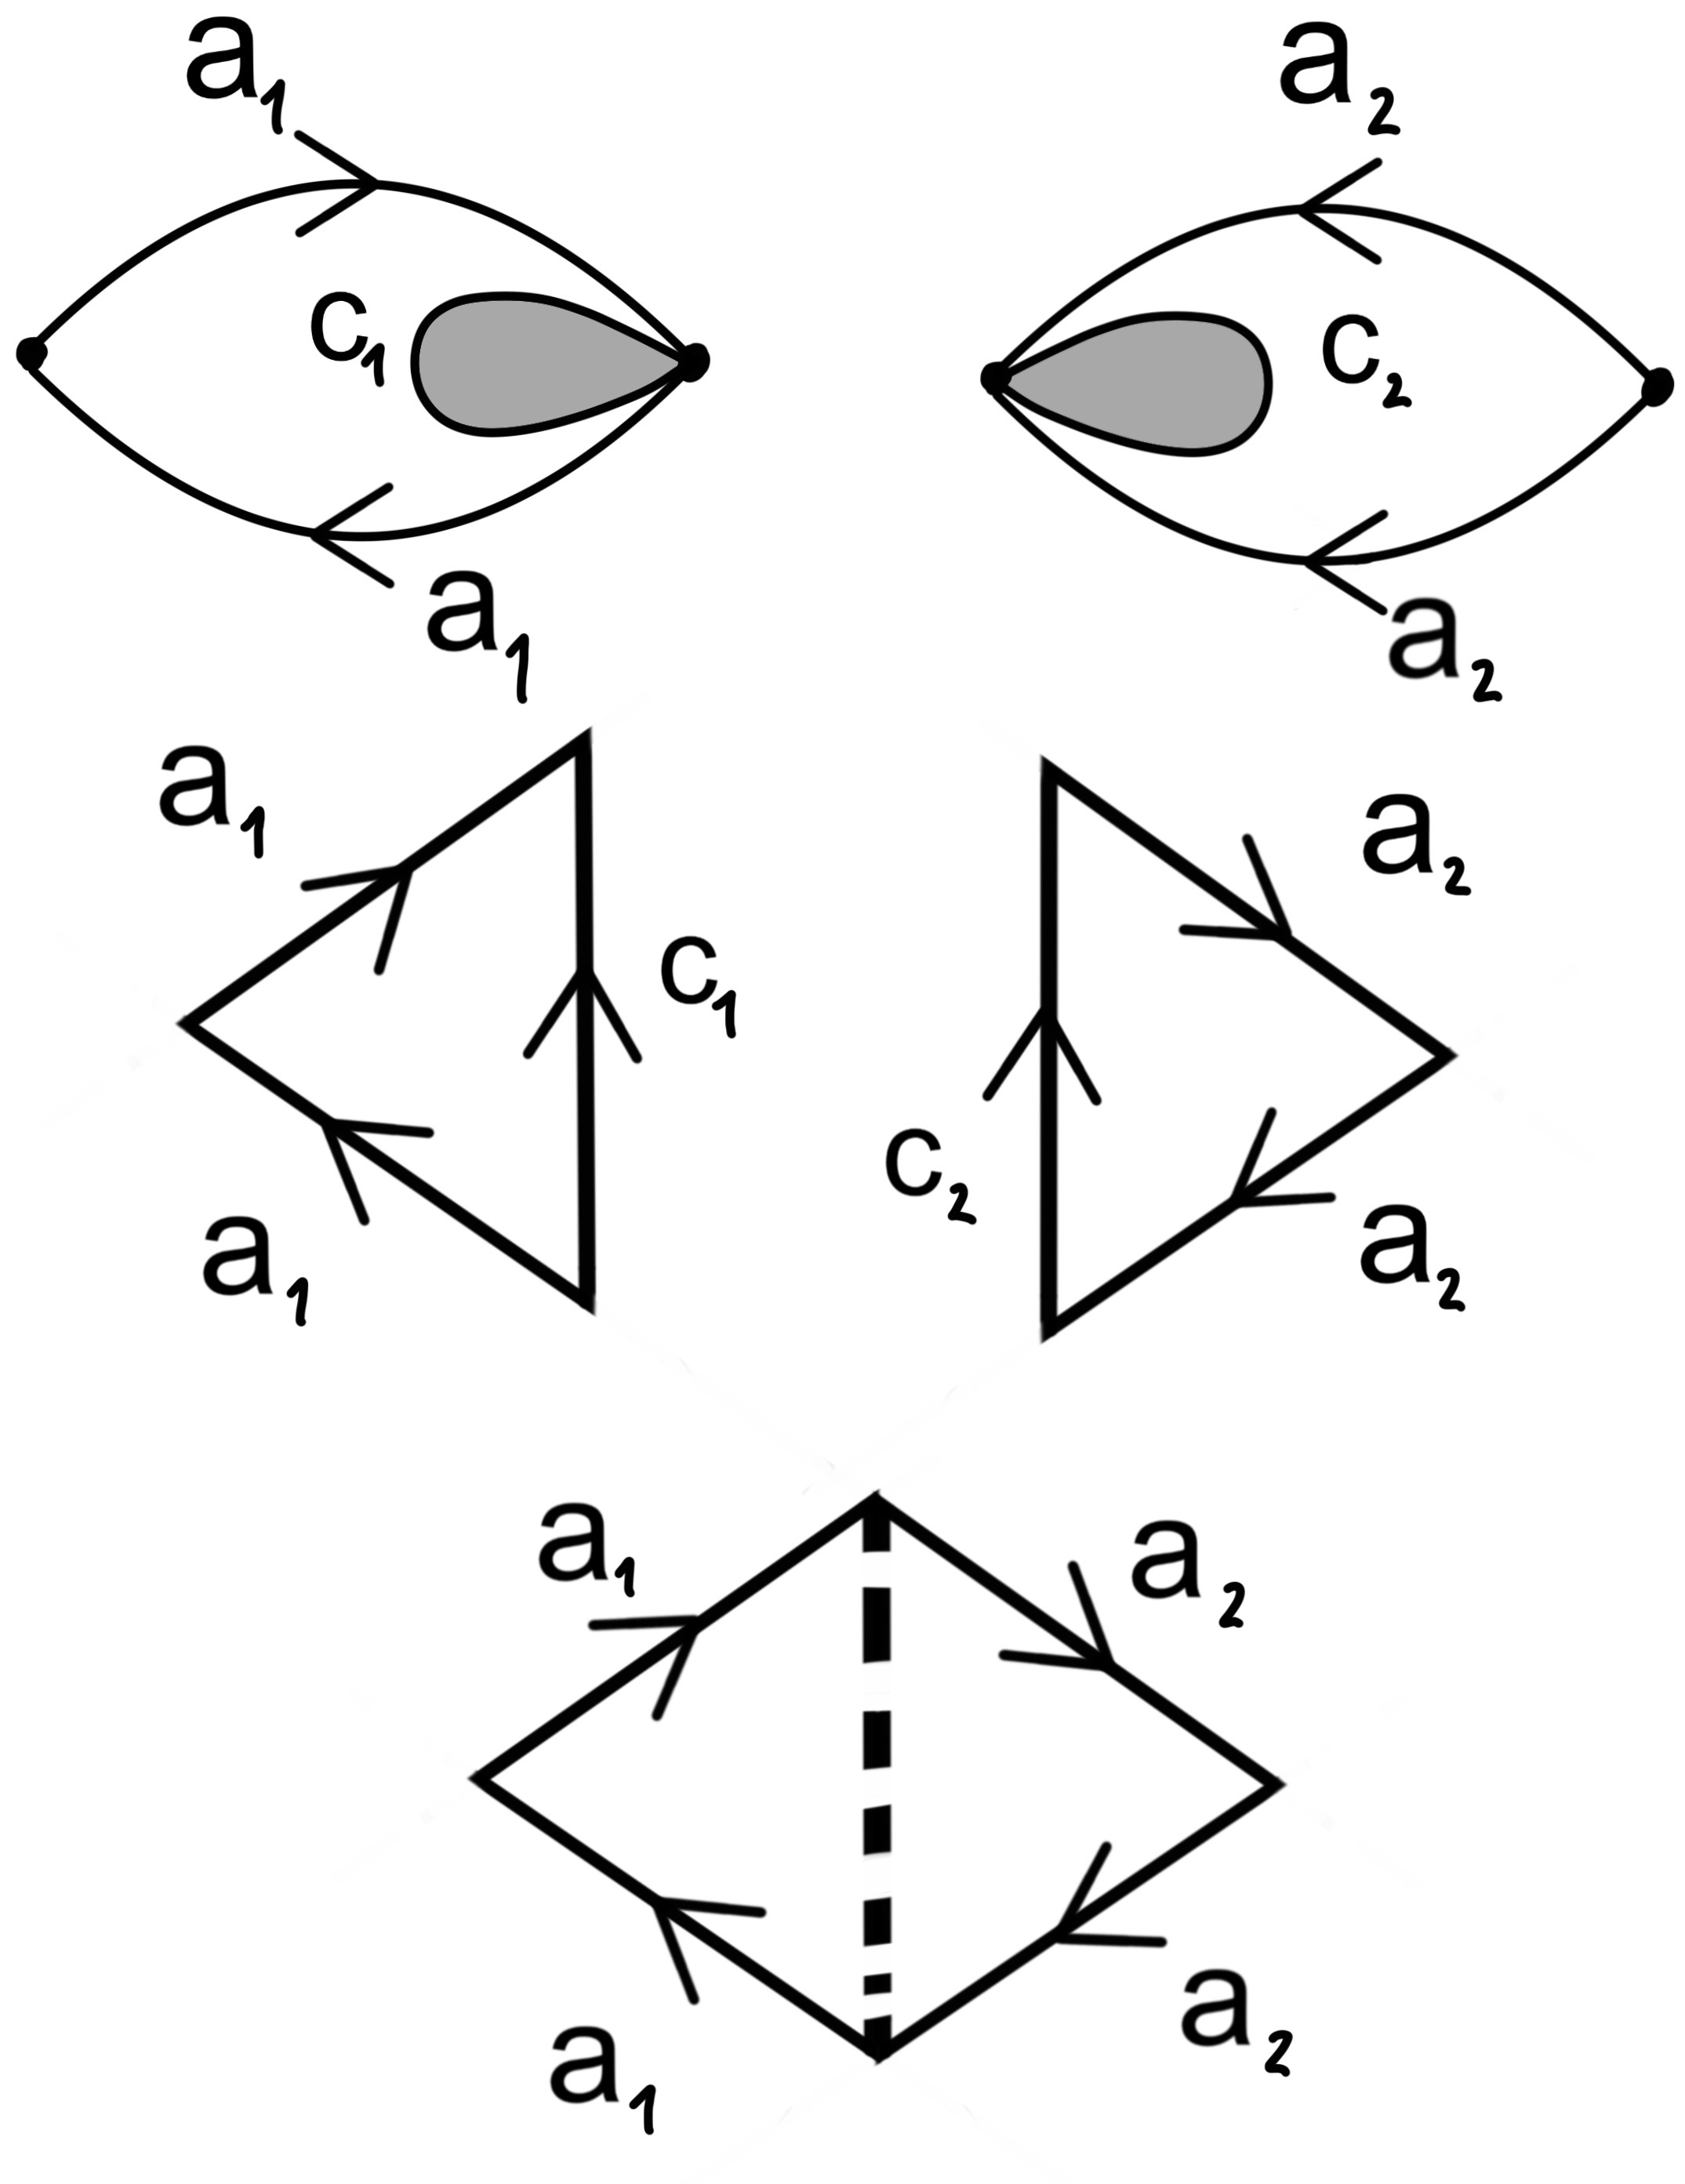
\includegraphics[width=0.3\linewidth]{imagenes/sumaconexa_planosp.png}
	\caption{Suma conexa de dos planos proyectivos}
	\label{fig:suma conexa de planos p}
\end{figure} 

\noindent \textbf{Suma conexa de esferas}
\\
En la figura \ref{fig:suma conexa de esferas} ilustramos la suma conexa de dos esferas. Curiosamente observamos que el resultado es otra esfera. Se puede comprobar que la esfera actúa como elemento neutro de la suma conexa.

\begin{figure}[h!]
	\centering
	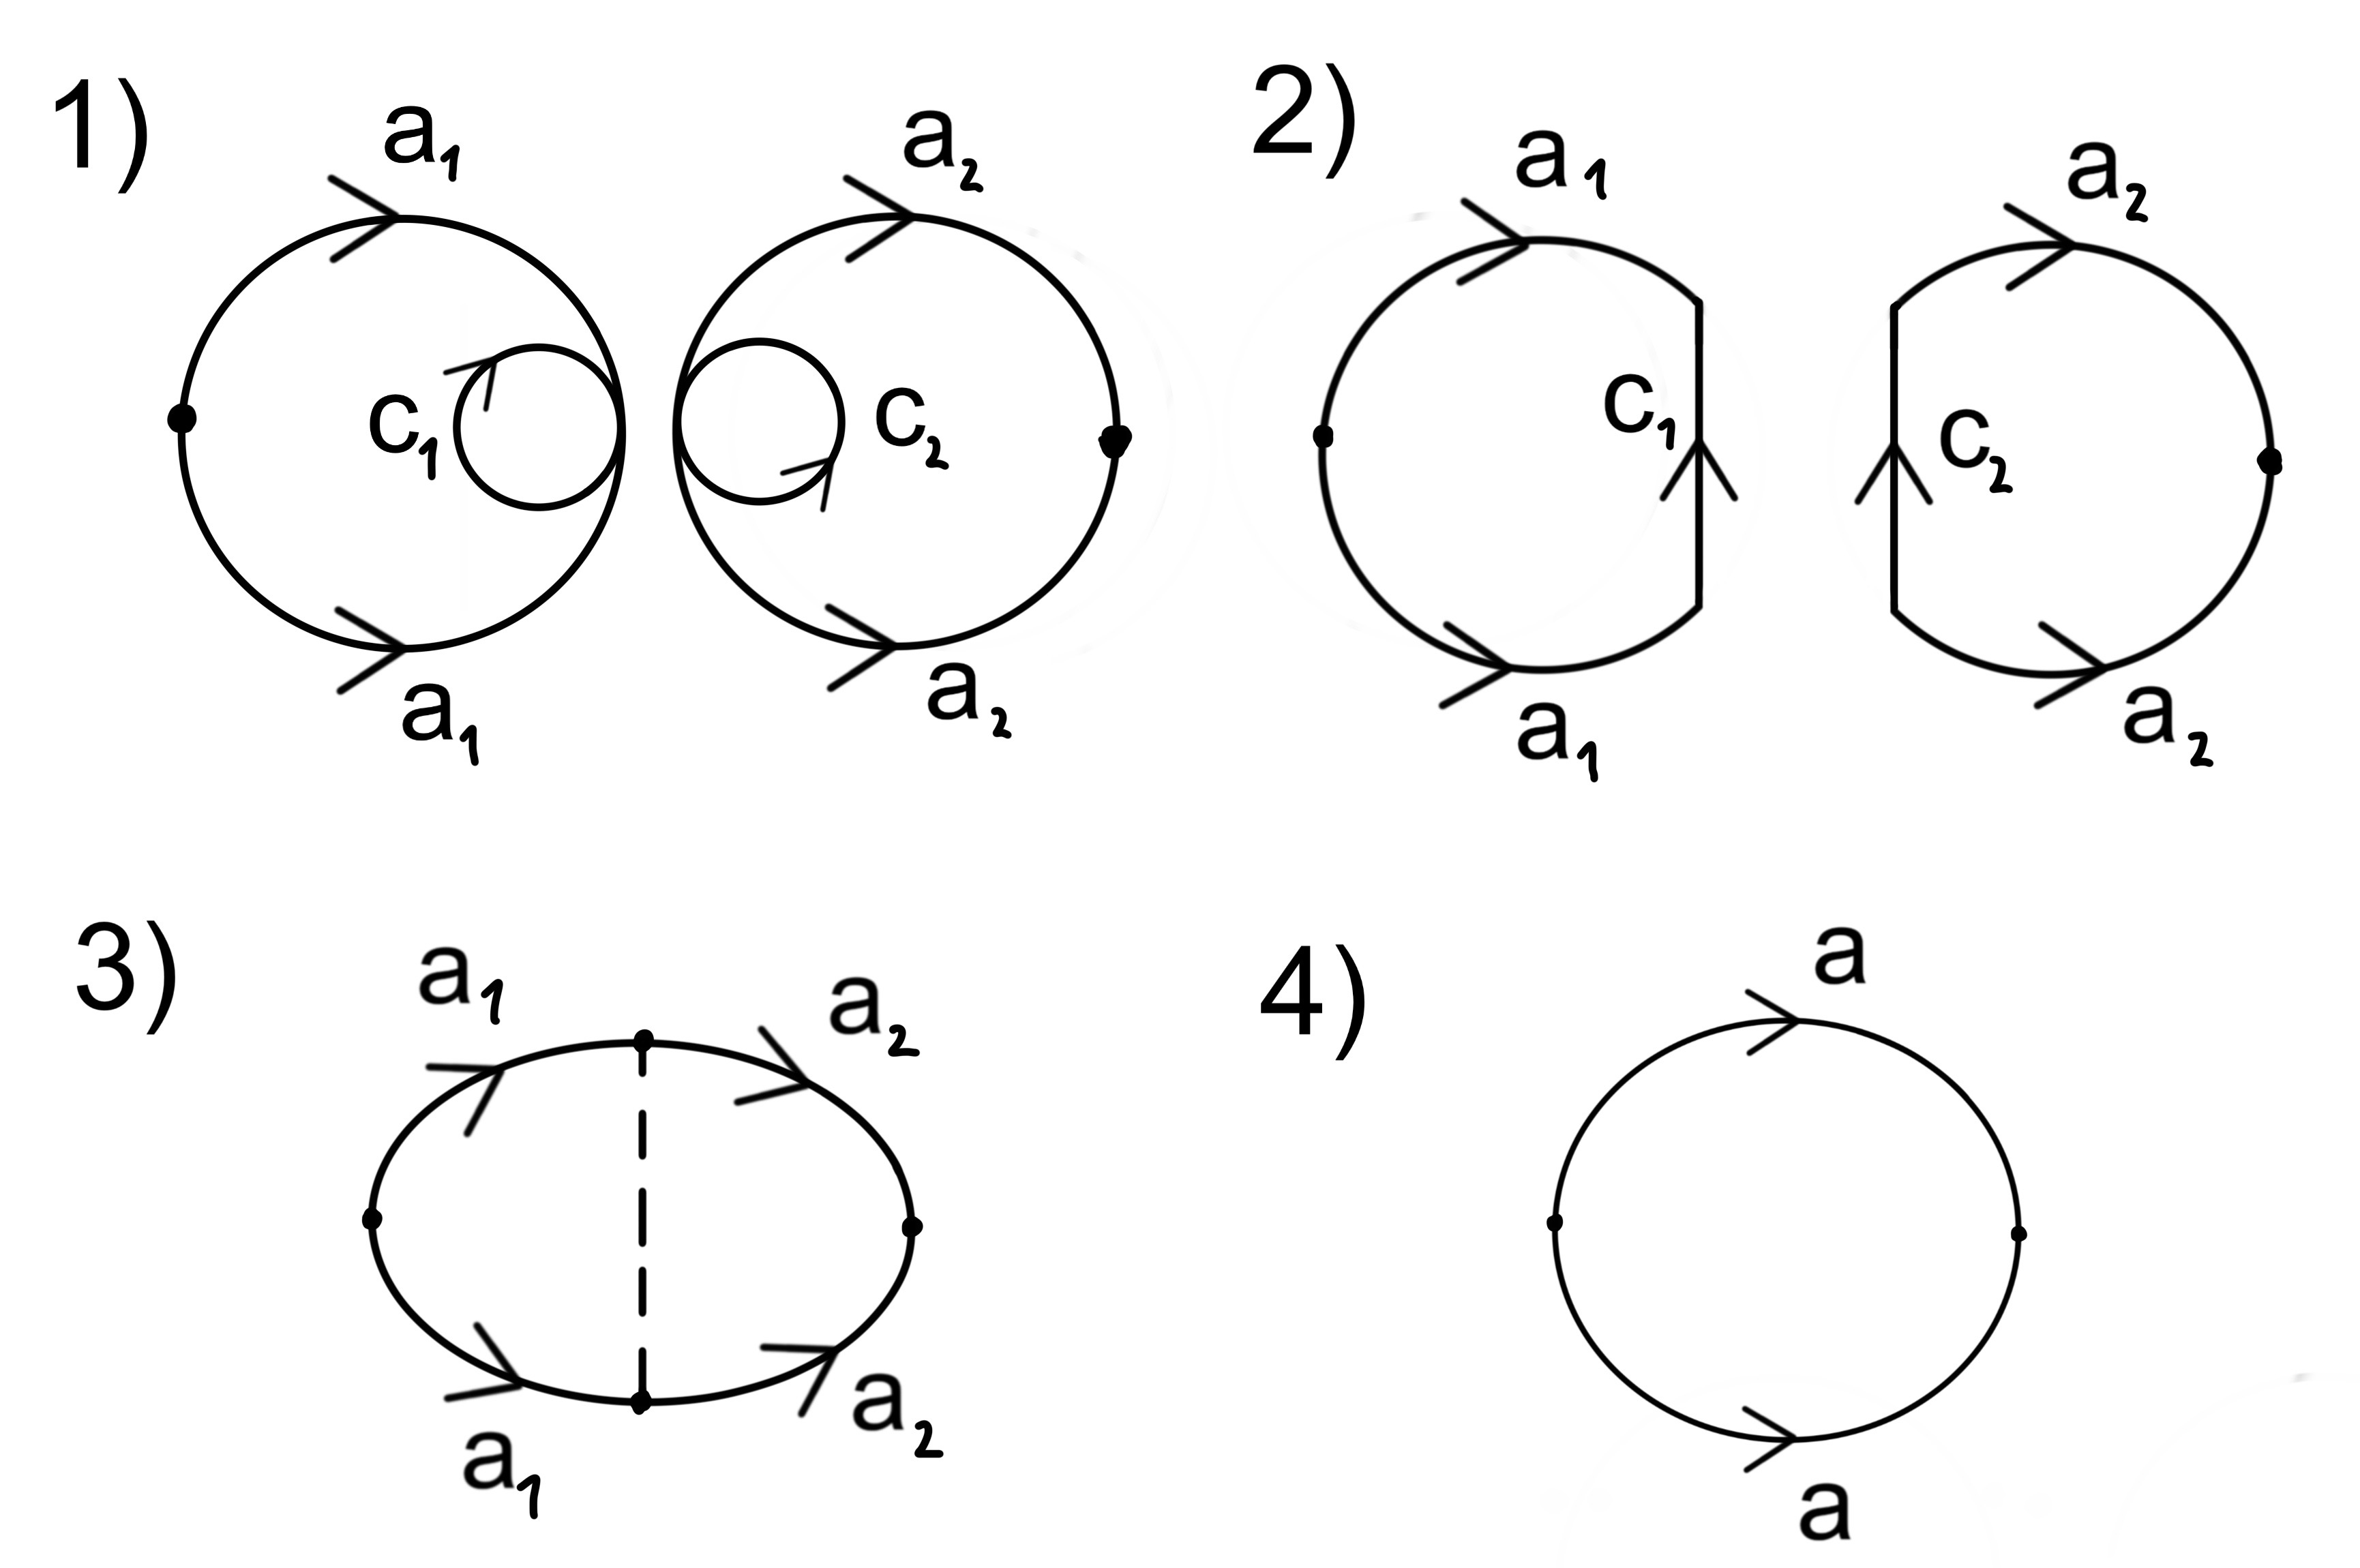
\includegraphics[width=0.5\linewidth]{imagenes/sumaconexa_esferas.png}
	\caption{Suma conexa de dos esferas}
	\label{fig:suma conexa de esferas}
\end{figure} 

Otra propiedad interesante de la suma conexa es que conserva la compacidad, i.e, si $S=S_1 \, \# \, S_2$, entonces $S$ será compacta si lo son $S_1$ y $S_2$. En los ejemplos de la suma de toros, planos proyectivos y esferas, basta con usar el lema \ref{lema:compacidadDePoligonos} para demostrarlo.

\subsection*{Expresiónes canónicas de sumas conexas}

Los ejemplos mencionados en la sección anterior proporcionan un método para describir sumas conexas arbitrarias de esferas, toros y planos proyectivos. Basta repetir los mismos procedimientos para comprobar que:

\begin{list}{-}{}
	\item La suma conexa de $ n $ esferas es igual a una esfera:
	\begin{align}\label{formacanonica:esfera}
		aa^{-1} 
	\end{align}
	\item La suma conexa de $ n $ toros se puede escribir como:
	\begin{align}\label{formacanonica:ntoros}
		a_1b_1a_1^{-1}b_1^{-1}a_2b_2a_2^{-1}b_2^{-1}...a_nb_na_n^{-1}b_n^{-1}
	\end{align}
	\item La suma conexa de $ n $ planos proyectivos se puede describir como: 
	\begin{align}\label{formacanonica:nplanosp}
	a_1a_1a_2a_2...a_na_n
	\end{align}
\end{list}
A las expresiones \ref{formacanonica:esfera},\ref{formacanonica:ntoros} y \ref{formacanonica:nplanosp} las llamaremos \textit{expresiones canónicas} de sus respectivas sumas conexas.

 
Antes de dar el asunto por concluido, veamos un último ejemplo de suma conexa:
\begin{lema}\label{lema:SumaDosPlanospEsKlein}
	La suma conexa de dos planos proyectivos es una botella de \textit{Klein}
	\begin{proof}
		En la demostración trataremos al plano proyectivo como el disco unidad identificando los puntos diametralmente opuestos.\\
		Seleccionamos del plano proyectivo el subconjunto $D = \left\{(x,y): |y|\geq\frac{1}{2}, |x|\leq\sqrt{1-y^2} \right\}$  homeomorfo al disco cerrado. Retiramos $ D $ como se muestra en la figura \ref{fig:planop sin D}, los segmentos discontinuos representan la frontera del disco por la cual se ha de realizar la suma conexa.
		\begin{figure}[h!]
			\centering
			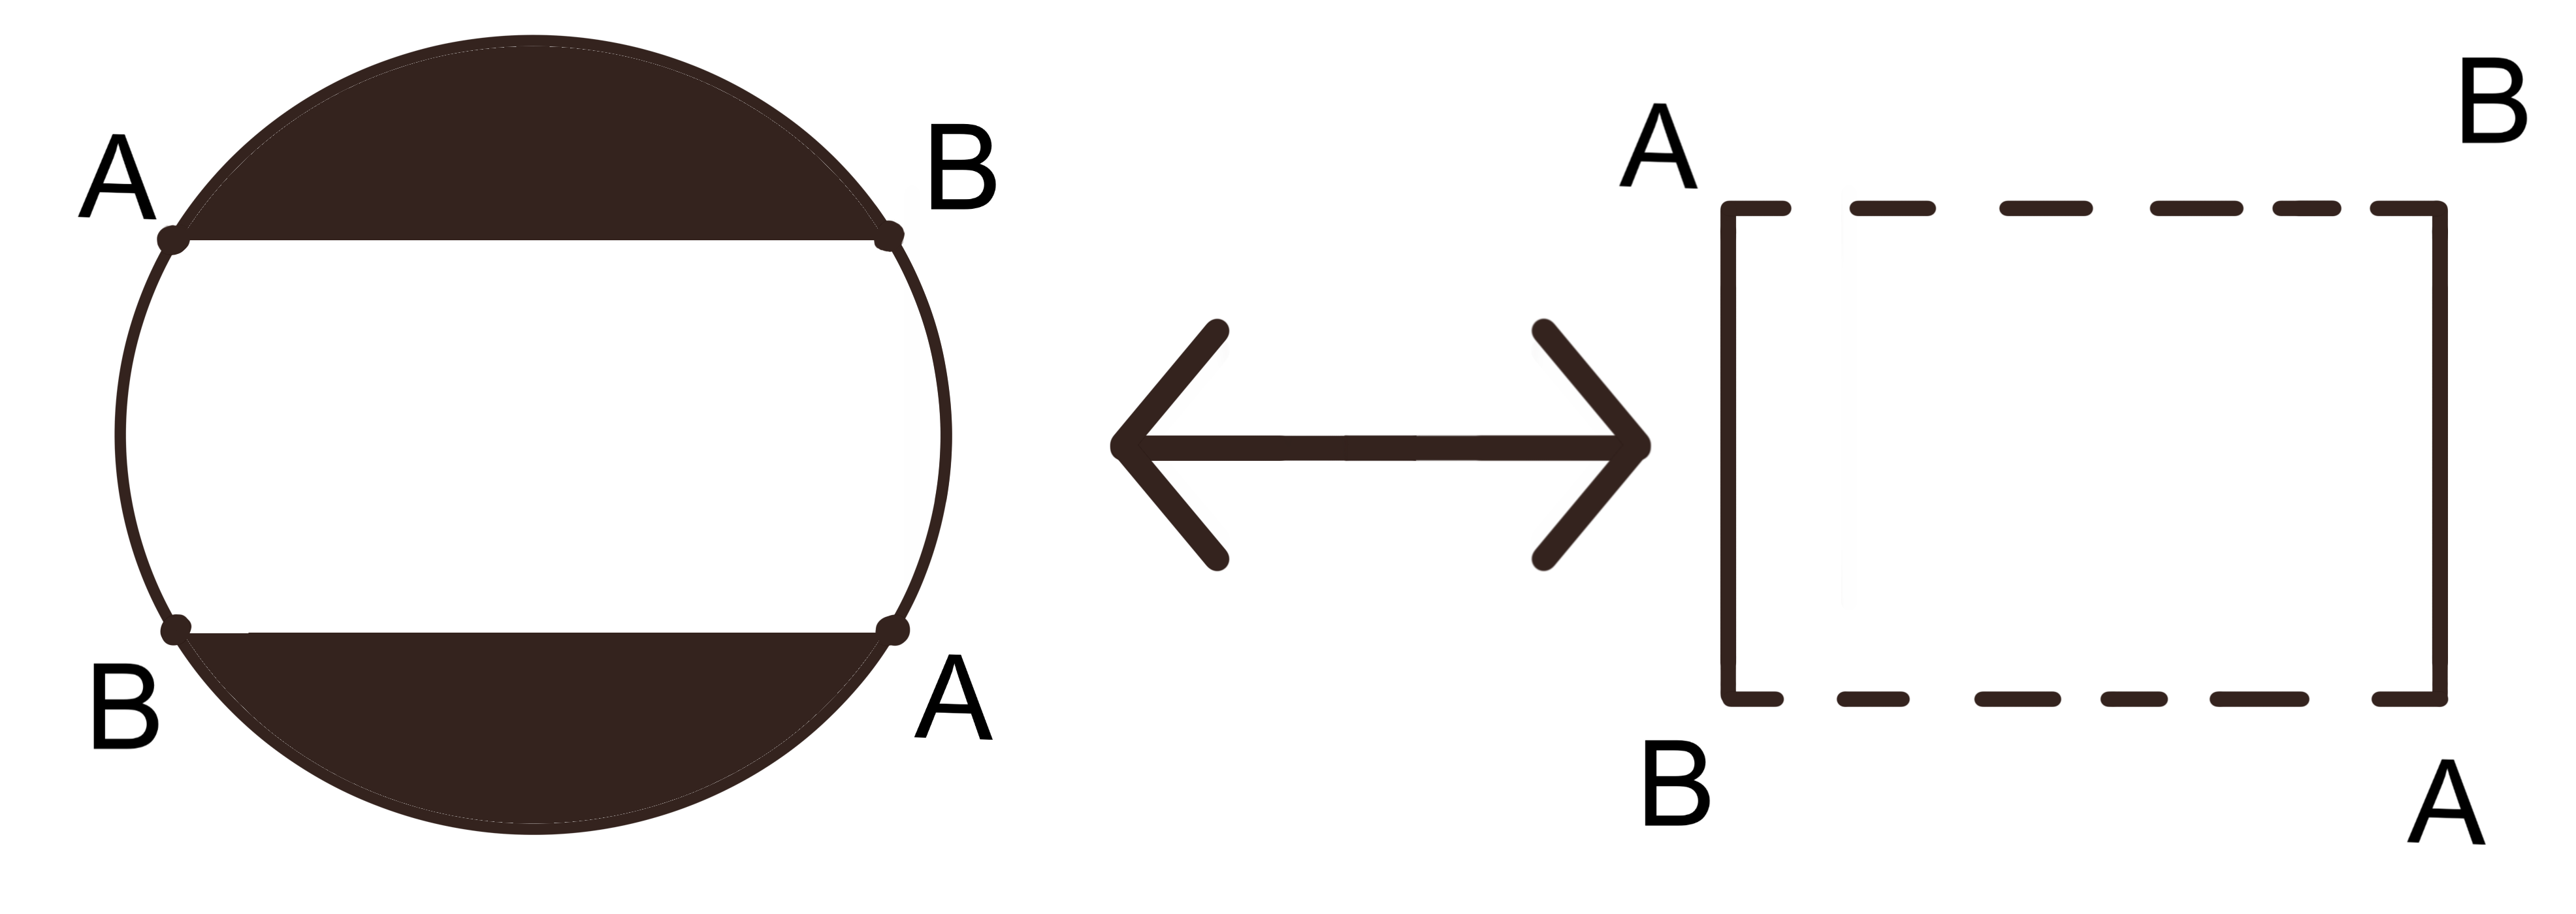
\includegraphics[width=0.4\linewidth]{imagenes/planop_sinD.png}
			\caption{Plano proyectivo menos un subconjunto homemorfo al disco cerrado}
			\label{fig:planop sin D}
		\end{figure} 
		
		Partiendo de dos planos proyectivos,  $I$ e $II$, retiramos el disco como en la figura \ref{fig:planop sin D}. Luego procedemos a identifcar ambos conjuntos como se indica en la figura \ref{fig:sumaconexadeppsEnLema}.
		
		\begin{figure}[h!]
			\centering
			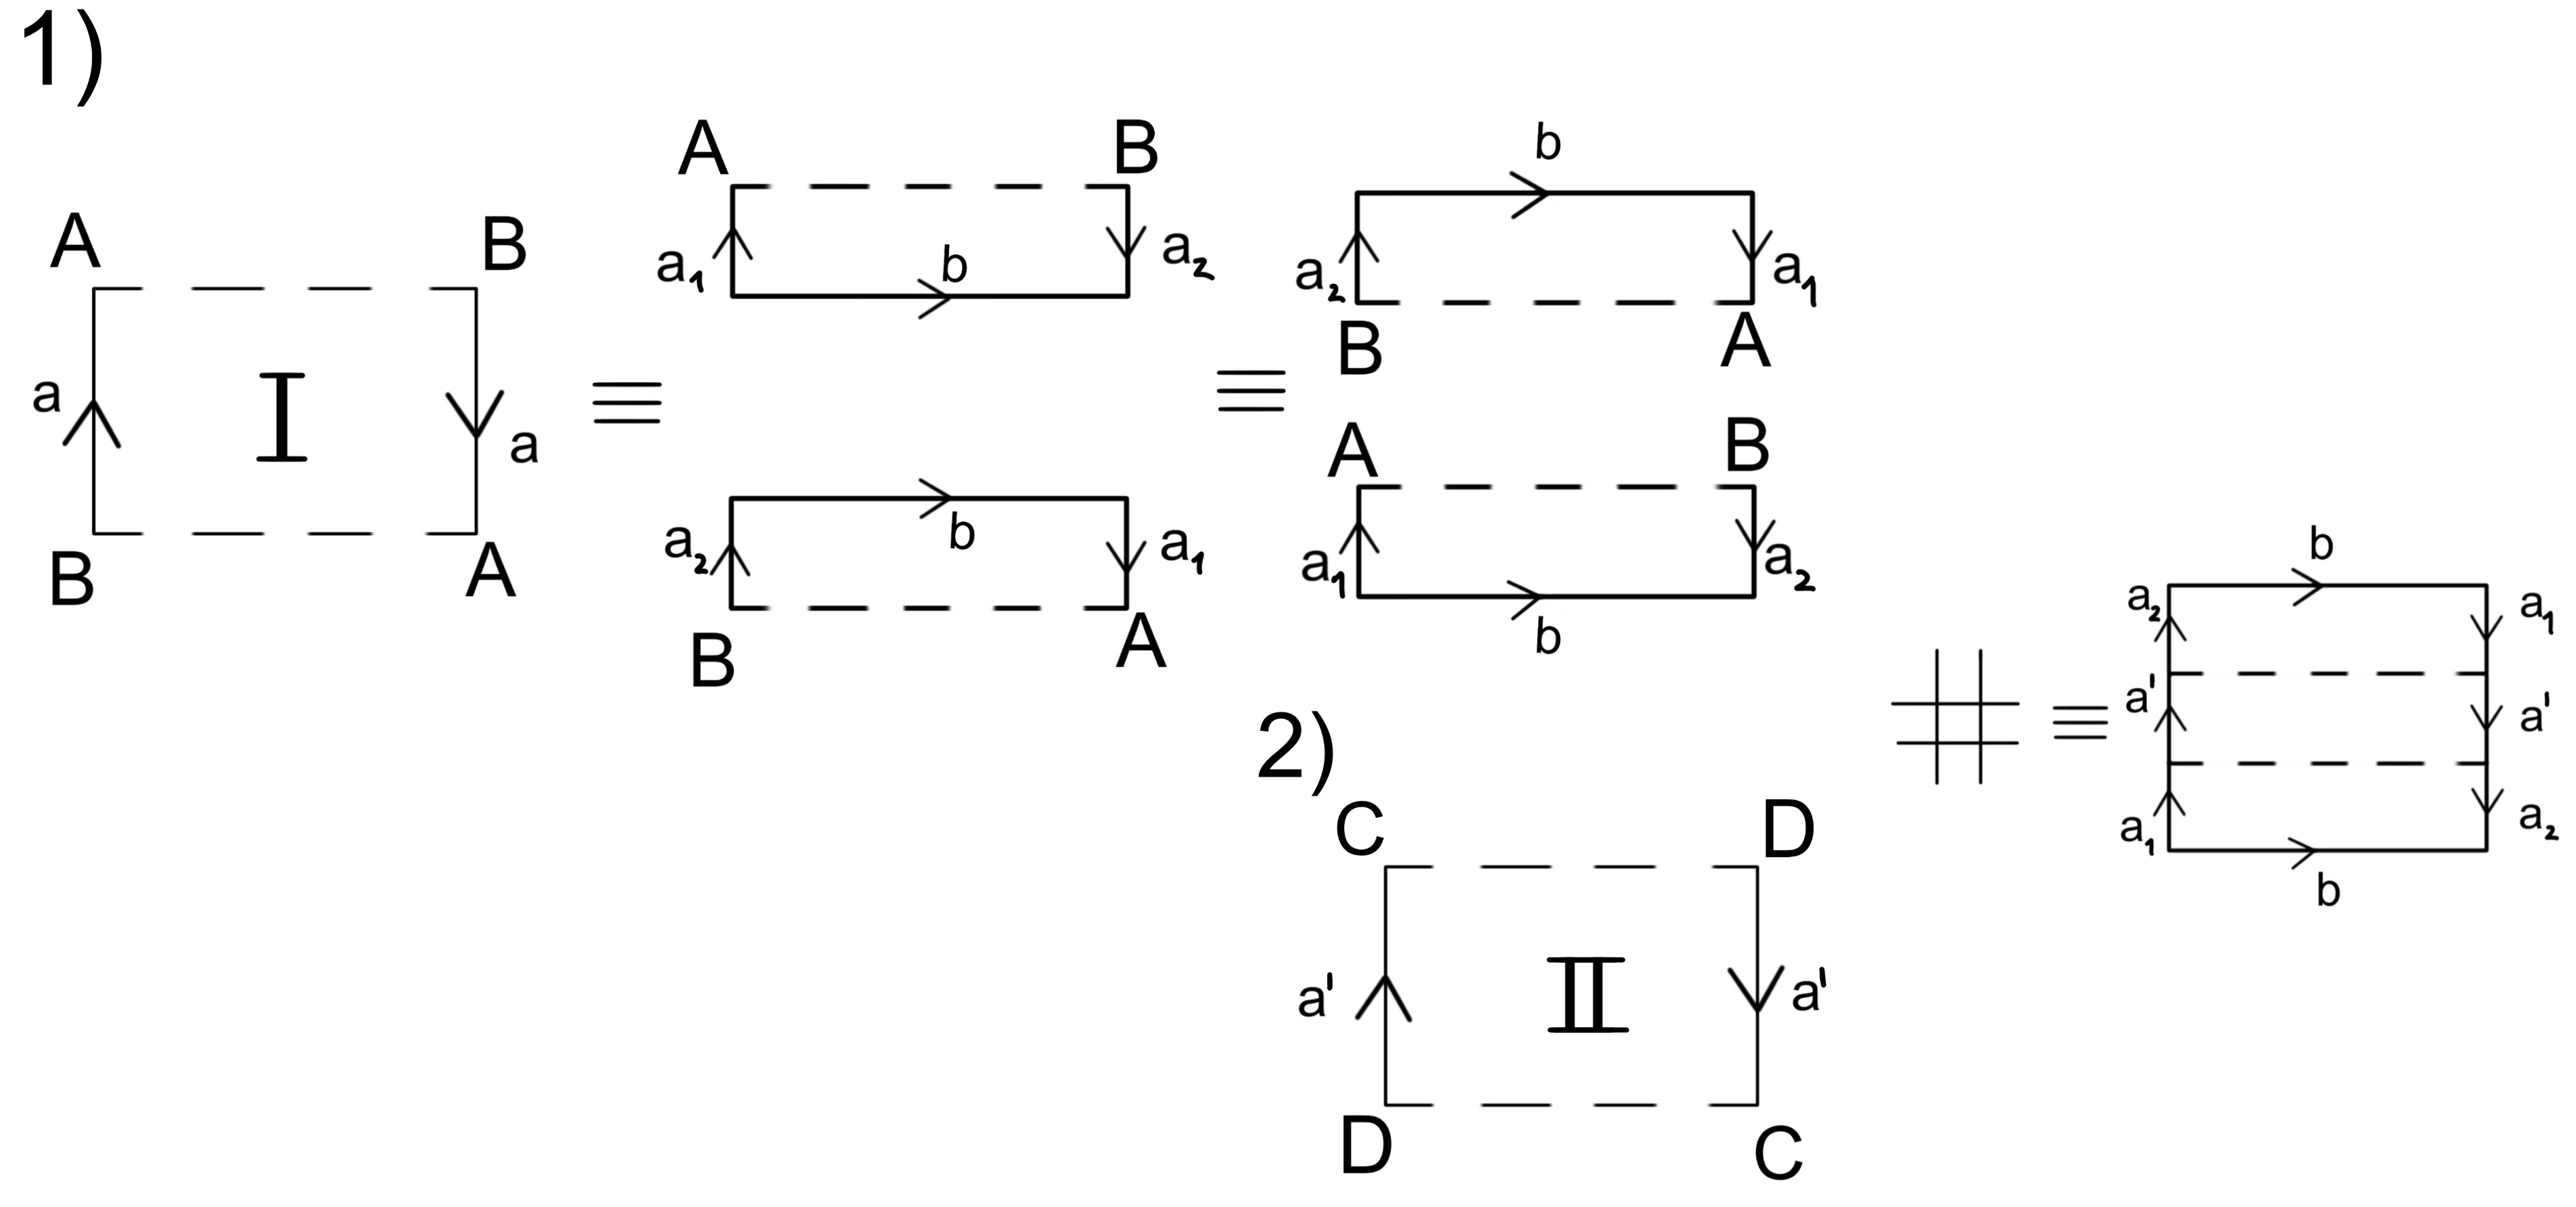
\includegraphics[width=0.8\linewidth]{imagenes/sumappsEnLema.png}
			\caption{Botella de \textit{Klein} = $ I \# II$}
			\label{fig:sumaconexadeppsEnLema}
		\end{figure} 
		La figura final obtenida  es una \textit{Botella de Klein}.
	\end{proof}
\end{lema}

El ávido lector se habrá dado cuenta de un detalle curioso de la demostración, retirar un disco de un plano proyectivo lo convierte en una banda de M\"obius!

\section{Triangulación de una superficie}
Una triangulación, en caso de existir, pretende expresar una superficie como un conjunto de triángulos identificados por las aristas. La noción de triangulación, \textit{a priori} inofensiva, será un ingrediente clave para poder manipular superficies compactas. Se define rigurosamente como:

\begin{defin}\label{defin:triangulacion}
	Una \textbf{triangulación} de una superficie compacta, $S$, consiste en subconjuntos cerrados, $\{T_1, ..., T_n\}$, que cubren a $S$ y en una familia de homeomorfismos, $\{\phi_1, ..., \phi_n\}$, que cumplen:
	\begin{align*}
	\phi_i: T'_i \longrightarrow T_i
	\end{align*}
	Donde $T'_i$ es un triángulo del plano $\mathbb{R}^2$.
	Además, se exige que para cualesquiera dos $T_i$ y $T_j$ con $i\neq j$, se cumpla una de las siguientes condiciones:
	\begin{itemize}
		\item 
		Son conjuntos totalmente disjuntos.
		\item 
		Comparten un vértice en común y solo eso.
		\item 
		Tienen toda una arista en común y solo eso.
	\end{itemize}
	Adicionalmente, llamaremos \textbf{vértice} a todo elemento de $S$ que se corresponde por algún $\phi_i$ con un vértice en el plano. Y llamaremos \textbf{arista} a todo subconjunto de $S$ que tenga por imagen una arista de algún $T'_i$.
\end{defin}


Intuitivamente, podemos pensar en una triangulación como una teselación por triángulos de una superficie dada. Estudiemos algunos ejemplos concretos para familiarizarnos con el concepto:

El toro se puede triangular como ilustra la figura  \ref{fig:toro triangulado}. Fijémonos que basta con definir una lista de triángulos, con sus respectivos vértices, para concretar una trinagulación. En la figura indicada la lista sería:
[Lista de triángulos]


\begin{figure}[h!]
	\centering
	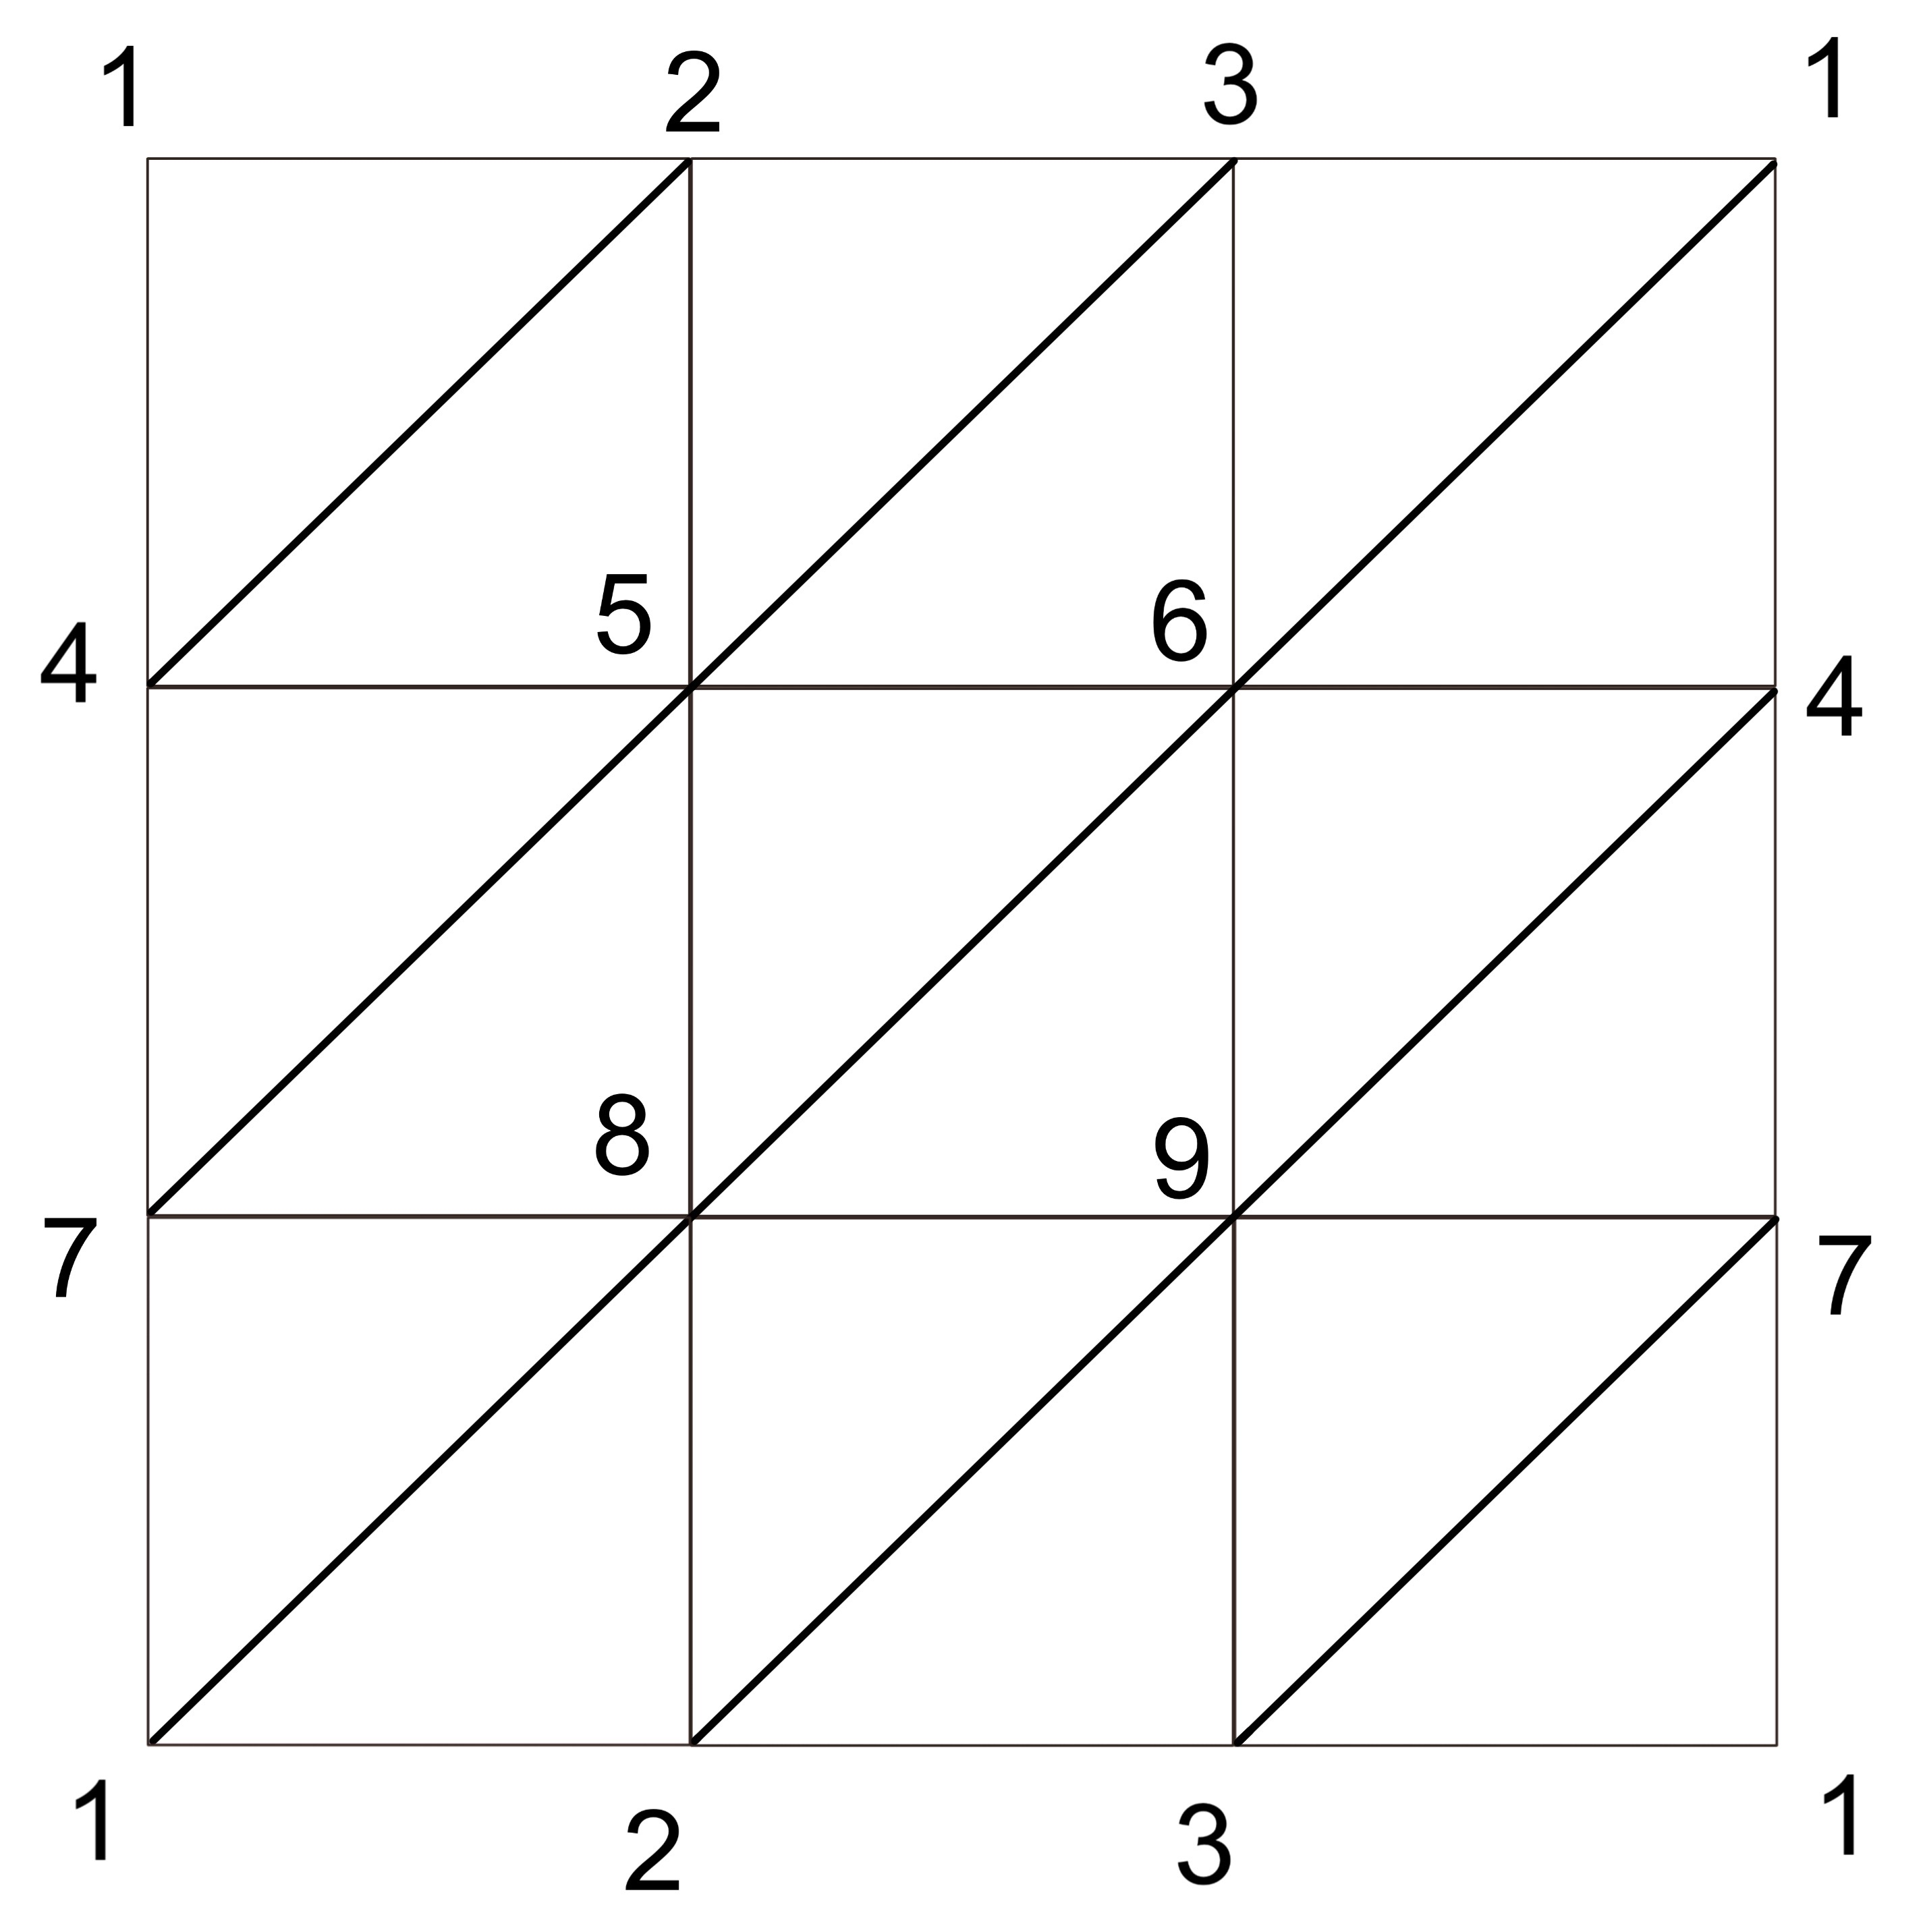
\includegraphics[width=0.3\linewidth]{imagenes/toro_triangulado.png}
	\caption{Triangulación del toro}
	\label{fig:toro triangulado}
\end{figure} 
En la figura \ref{fig:no triangulaciones} señalamos un par de intentos de simplificar la triangulación del toro. Sin embargo, notemos que ninguna de las dos imágenes son triangulación del toro. La primera, aunque triangulación, no es homeomorfa al toro; La segunda ni siquiera satisface las condiciones de triangulación.


\begin{figure}[h!]
	\centering
	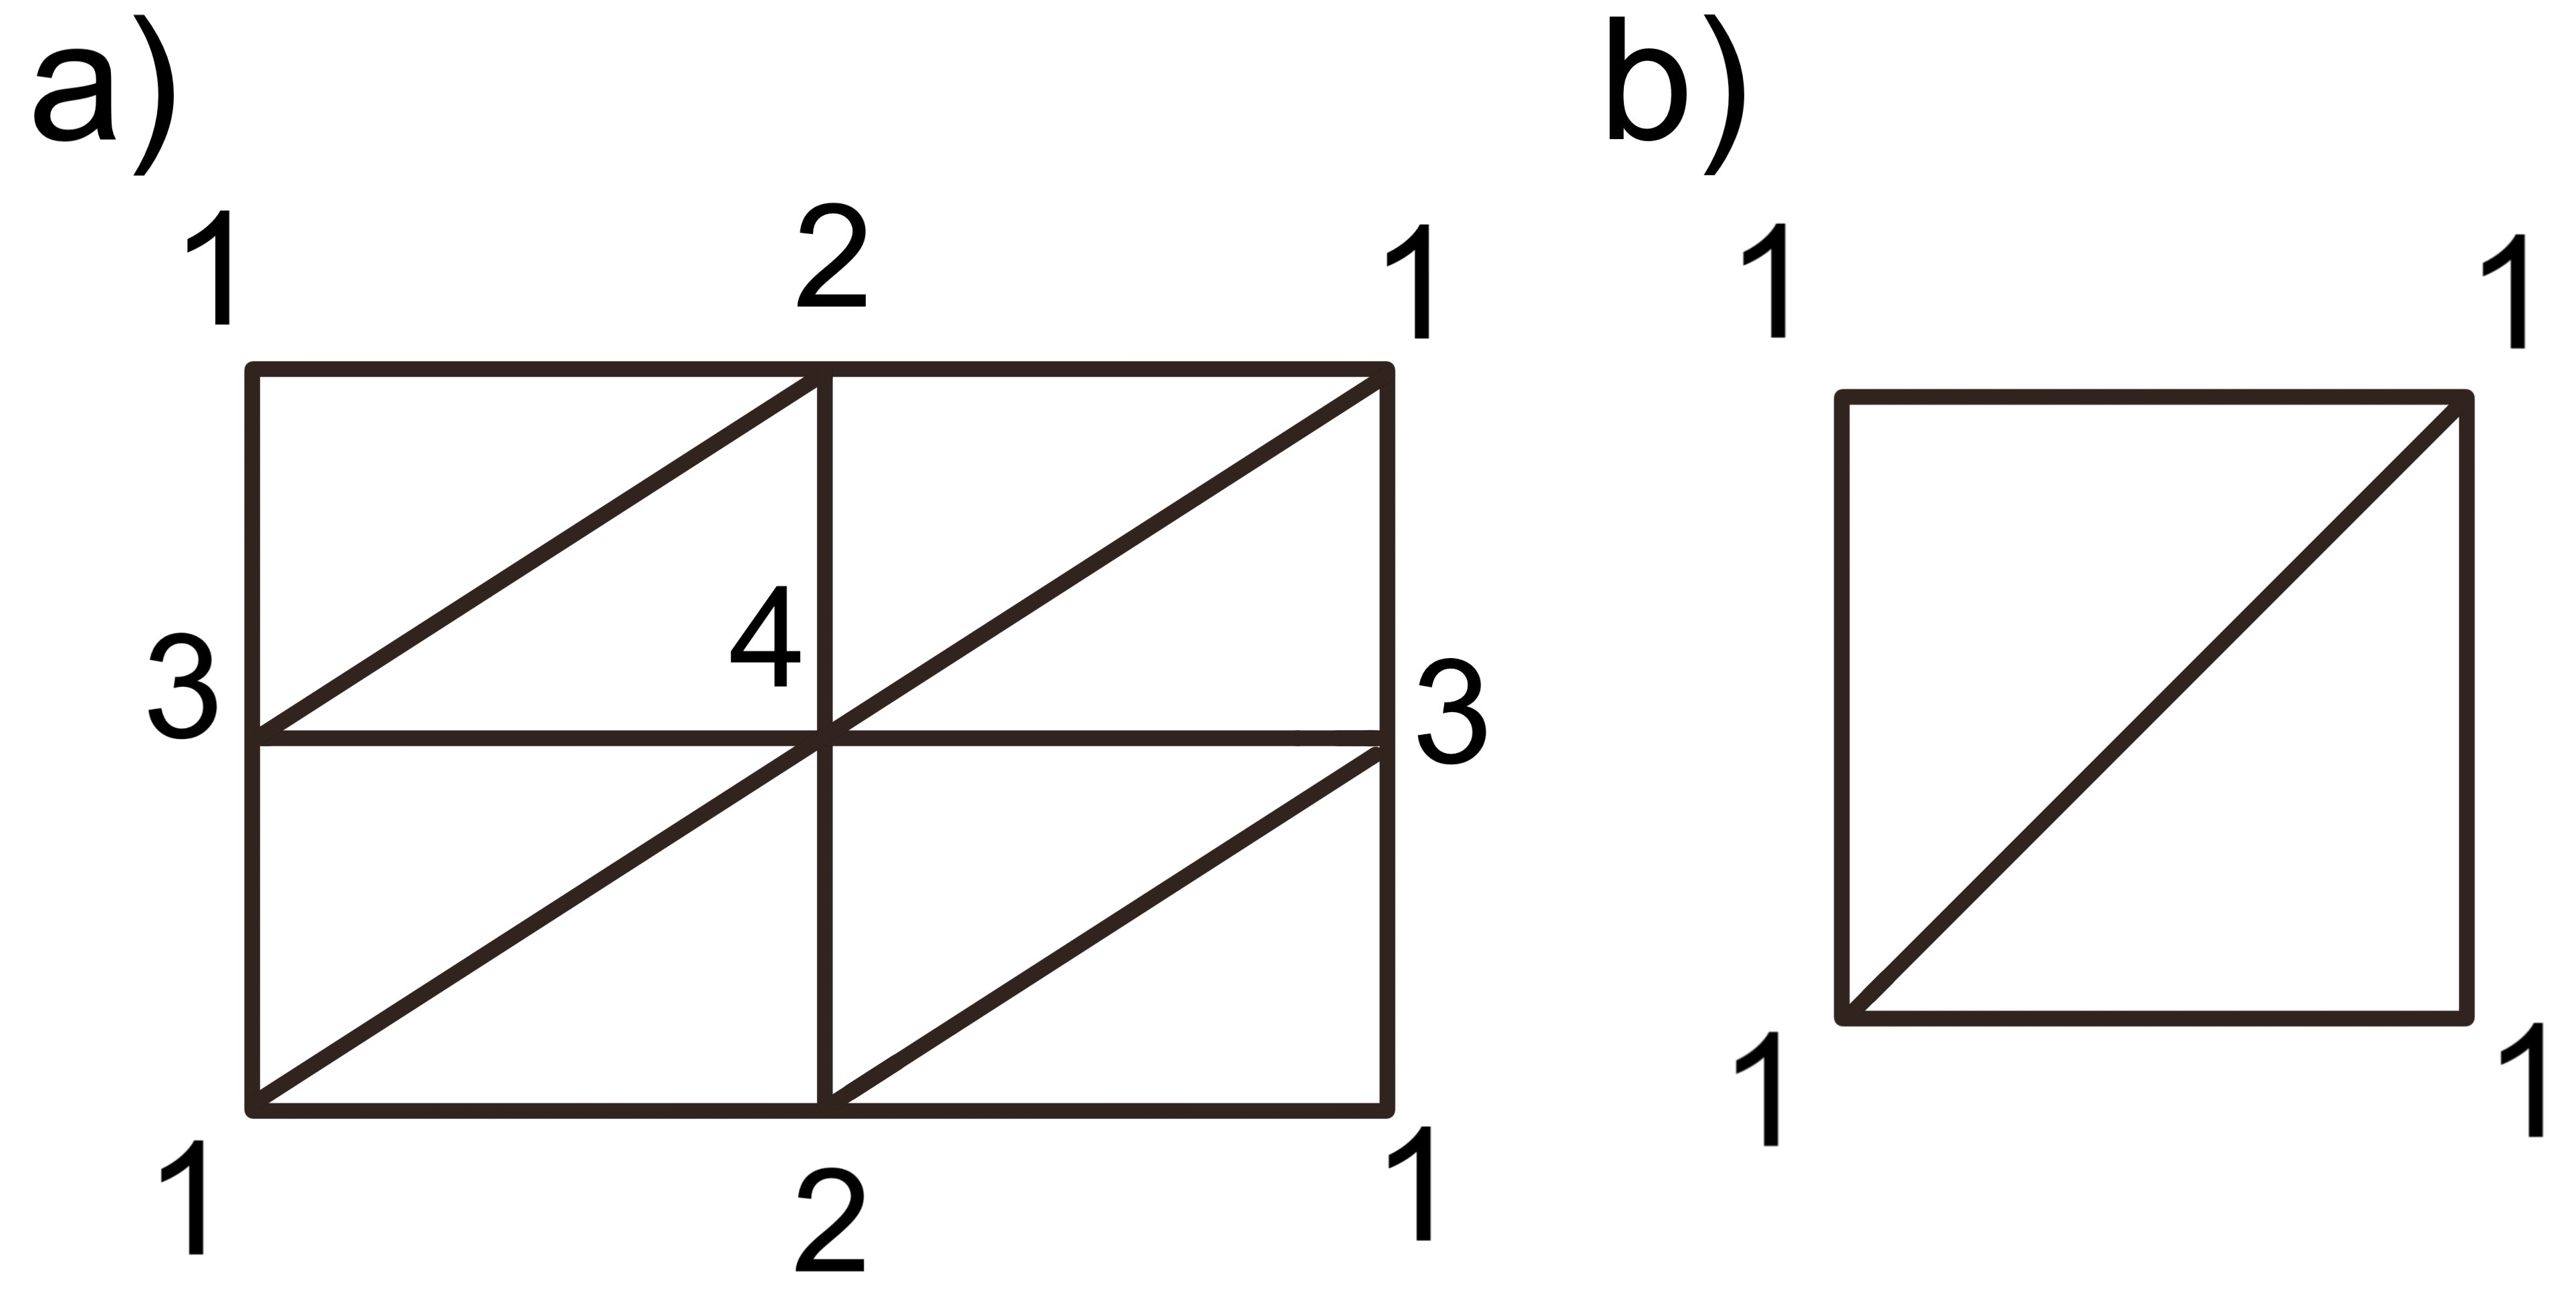
\includegraphics[width=0.5\linewidth]{imagenes/no_triangulaciones.png}
	\caption{Ejemplos de cosas que no son triangulaciones}
	
	\label{fig:no triangulaciones}
\end{figure} 


Para el caso del plano proyectivo, se propone en la figura \ref{fig:plano proyectivo triangulado} una triangulación.
\begin{figure}[h!]
	\centering
	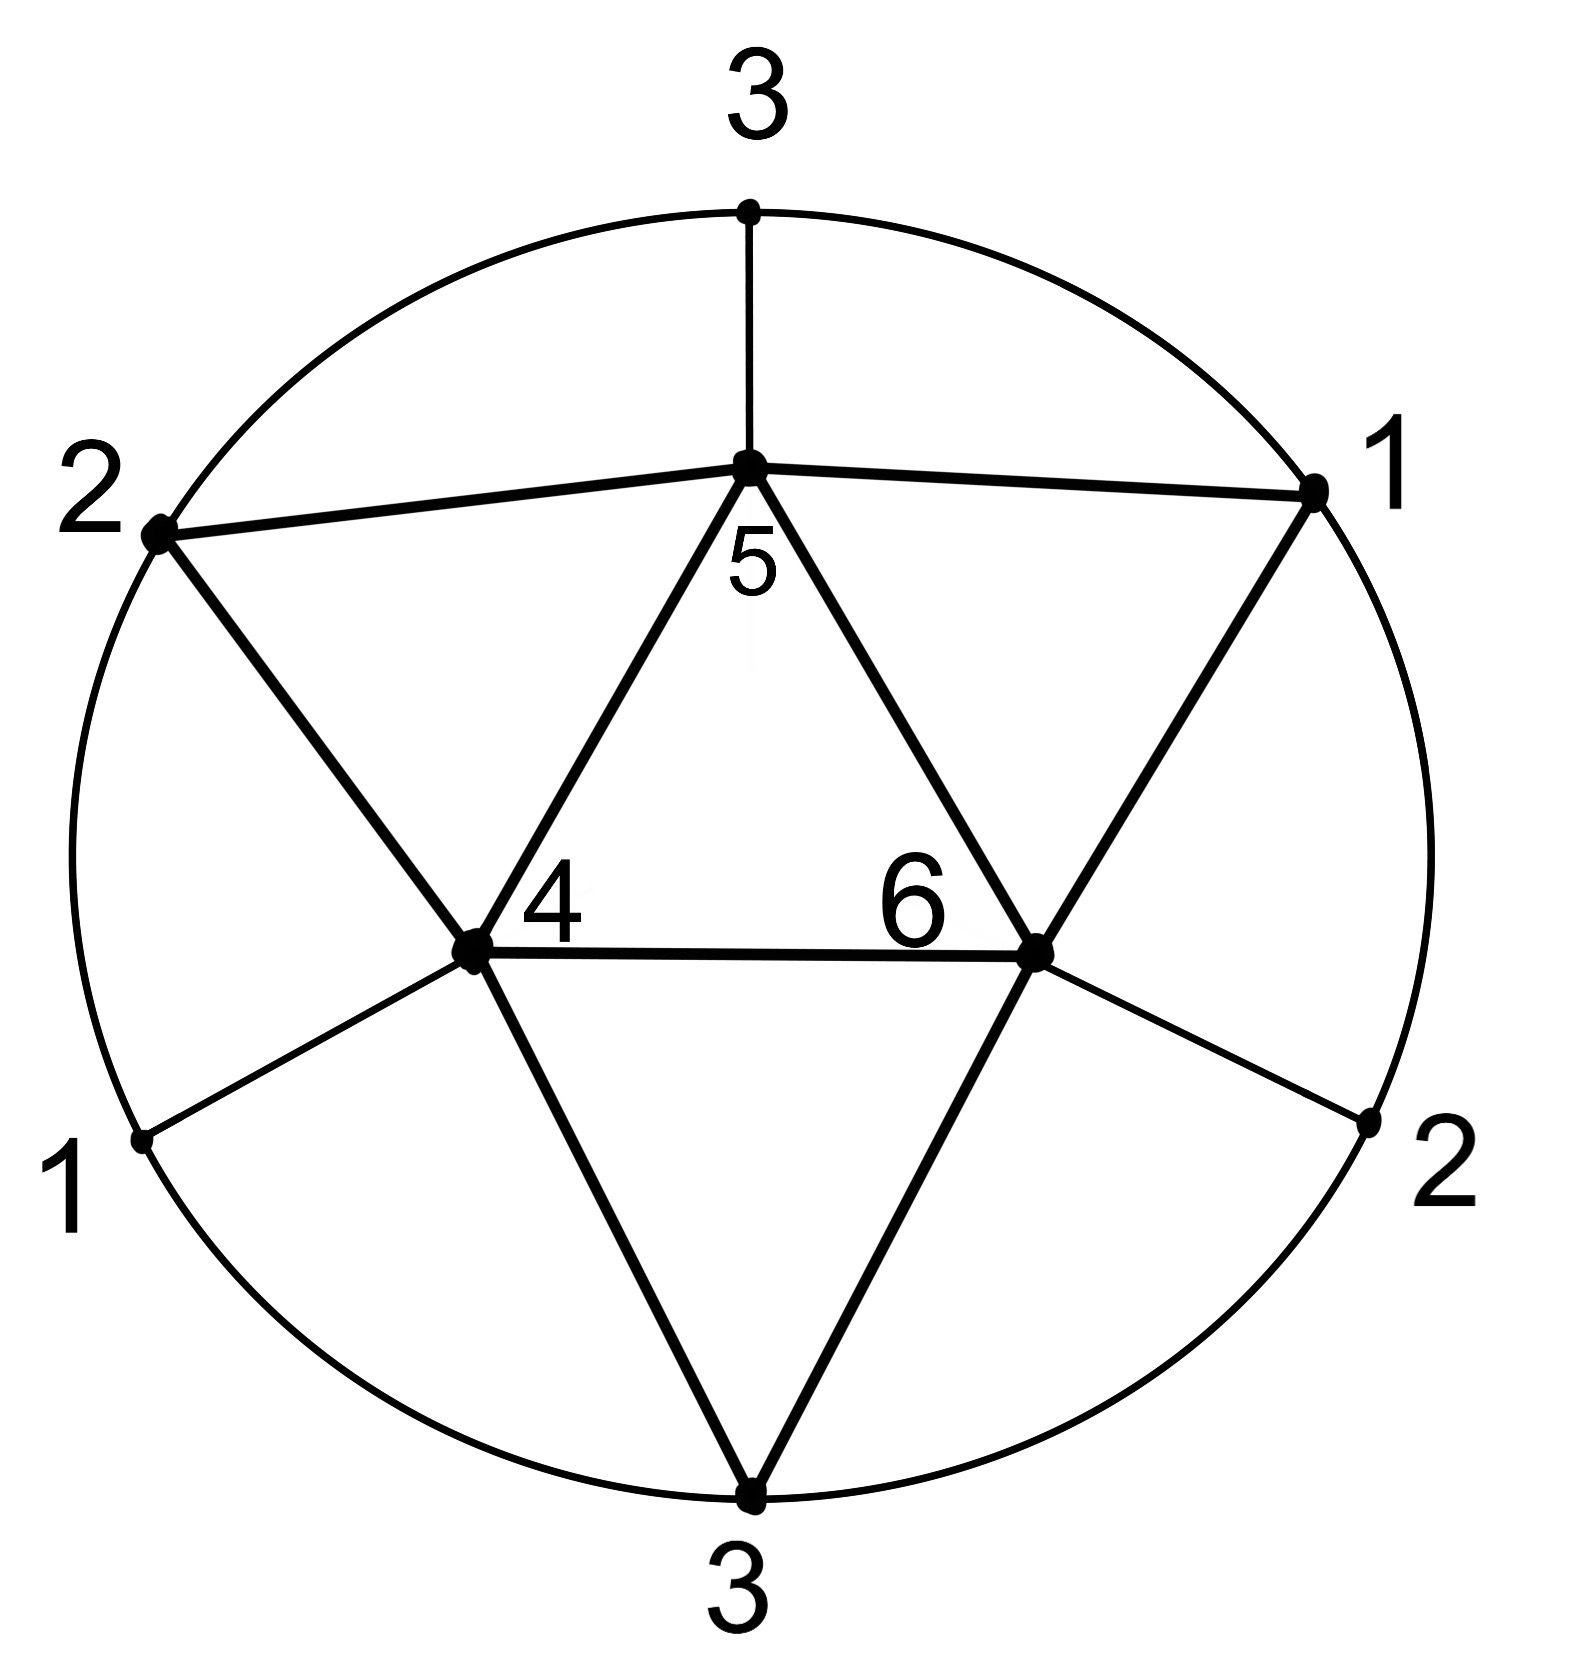
\includegraphics[width=0.3\linewidth]{imagenes/planop_triangulado.png}
	\caption{Triangulación del plano proyectivo}
	\label{fig:plano proyectivo triangulado}
\end{figure} 


\subsection*{Resultados sobre la triangulación}

Primero, veamos un par de lemas que nos enmarcan el comportamiento de las triangulaciones:

\begin{lema}\label{lema:lema1detriangulacion}
	Sea $S$ una superficie triangulable entonces una arista lo es de exactamente dos triángulos.
	\begin{proof}
		TODO: En proceso, escribirla si hiciese falta\\
		Si un punto de una arista pertenece a n triángulos => existe entorno del punto que está contenido dentro de estos n triángulos disjuntos y solo comparten la arista.\\
		Una bola no puede ser homeomorfa a nada que no sea n=2.
	\end{proof}
\end{lema}


\begin{lema}\label{lema:lema2detriangulacion}
	Sea  $S$ una superficie triangulable y $v\in S$ un vértice en esa triangulación, entonces podemos ordenar el conjunto de todos los triángulos con vértice $v$ cíclicamente,  $T_0, T_1, ..., T_n = T_0$, de manera que $T_i$ y $T_{i+1}$ tienen toda una arista en común para todo $0\leq i\leq n-1$.
	\begin{proof}
		TODO: En proceso, escribirla si hiciese falta\\
		Que se puede conseguir es consecuencia de \ref{lema:lema1detriangulacion}.\\
		Que es único tengo que mirarlo en el libro
	\end{proof}
\end{lema}

La triangulación nos servirá más adelante como herramienta potentísima para demostrar el teorema de clasificación de superficies compactas. Comprobaremos que con ella podremos expresar cualquier superficie topológica compacta, por abstracta que sea, como un conjunto de triángulos en 
Intuitivamente, podemos pensar en la triangulación como una teselación por triángulos de una superficie. Para el caso de una esfera o un toro uno puede imaginarse tales teselaciones

La triangulación compone una herramienta potente para el manejo de superficies compactas. Comprobaremos más adelante que nos permite manipular la superficie como si se tratara de triángulos en $\mathbb{R}^2$. Sin embargo, primero es necesario probar que \textit{de facto} existe tal triangulación, requisito que parece especialmente intimidante para el caso de conjuntos abstractos. Por suerte, el matemático Tibor Radó demostró un teorema que nos garantiza que toda superficie compacta es triangulable. Enunciamos el teorema sin, lamentablemente, dar demostración.

\begin{teor}{Teorema de triangulación}\label{teor:teoremaDeTriangulacion}	
	
	Toda $S$ superficie compacta es triangulable.
\end{teor}

Con este teorema concluimos el arsenal de herramientas que nos hará falta para emprender la demostración del teorema de clasificación de superficies compactas.






\chapter{Clasificación de superficies compactas}

\begin{teor}{Teorema de clasificación de superficies compactas}\label{teor:teoremadeclasificacion}
	
	Toda superficie compacta es homeomorfa a una esfera, a una suma conexa de toros o una suma conexa de planos proyectivos.
\end{teor}
\begin{proof}
Da proof
\end{proof}

\chapter{Hacia las superficies no compactas}
[Complicaciones, citar resultados para superficies con borde]

[Introducir finales y frontera ideal]

[Demostrar algunos, citar otros, lemas de fronteras ideales]

[Tma de Kerekjartos sobre clasificación]

[Relación de espacios totalmente inconexos, separables (cjto denso 
numerable) y compacto con el Cjto de Cantor]

[Construcción de Ian Richards dando una superficie a cada posible frontera ideal]

\chapter{Algunos resultados que no sé si incluiremos}
Cosas que empecé a escribir pero que probablemente no haga falta incluir en el TFG. Son definiciones elementales de topo y algunos lemas.

\begin{defin}
	Un conjunto $\mathcal{X}$ es no conexo si existen dos  conjuntos cerrados, $\mathcal{X}_1$ y $\mathcal{X}_2$, tal que $\mathcal{X}=\mathcal{X}_1\cup\mathcal{X}_2$ y $\mathcal{X}_1\cap\mathcal{X}_2=\emptyset$.
\end{defin}
\begin{defin}
	Un conjunto $\mathcal{X}$ se dice conexo si no cumple la definición anterior.
\end{defin}
[Def de topo cociente]
[Compacto va a compacto por f cont, conexo va a conexo]


\begin{lema}{El pseudolema más útil de toda la topología}
	
	Al dilatar, comprimir, trasladar y cortar-identificar una figura, el objeto obtenido es homeomorfo al inicial. ¿Por qué?, se pregunta un matemático, porque todas las transformaciones son continuas. (¿Incluir en el TFG en tono seriesisímo?) 
\end{lema}
\begin{lema}\label{lema:sumaconexa}
	Para verificar que la suma conexa está bien definida hace falta aclarar varios puntos.
	\begin{enumerate}
		\item 
		Tenemos que asegurar la existencia de un subconjunto homeomorfo a un disco.
		\begin{proof}
			Tomamos un punto $p\in S_i$ cualquiera. Como $S_i$ es una 2-variedad, entonces existe un homeomorfismos $g$ que manda un entorno, $U$, del punto $p$ al círculo abierto. 
			
			Tomamos $E_{\frac{1}{2}}$ el disco cerrado de radio $\frac{1}{2}$, y $U'= g^{-1}(E_{\frac{1}{2}})$. Tenemos que $g\mid_{U'}$ es un homeomorfismo de un subconjunto de $S_i$ a $E_{\frac{1}{2}}$ que a su vez es homeomorfo al disco cerrado de radio 1. 
		\end{proof} 
		\item 
		Segundo, tenemos que asegurarnos que existe un tal $\psi$ homeomorfismo:
		\begin{proof}
			Utilizando los $g$ anteriores basta ver que  $g(fr(D_i))=fr(E^2)$, y luego componer las funciones para construir un homeomorfismo entre las fronteras.
		\end{proof}
		\item 
		Tercero, habría que comprobar que, en efecto, el objeto obtenido es una superficie. Es decir, comprobar que todo punto tiene un entorno homeomorfo al disco abierto, que el espacio es T2 y que es conexo.
		\begin{proof}
			Ideas (hace falta formalizarlo?)
			1. Entorno homeomorfo a la bola: Tenemos que comprobarlo para los ptos frontera. Esta dems es engorrosa: Basta quizás con ver que localmente podemos tratar a los puntos de la frontera como si estuviesemos en R2, observando las construccioines de homeomorfismos podemos concluir que se puede crear un entorno homeomorfo a una bola al pegar dos semicírculos de cada superficie (vistas en R2 localmente). 
			2. Conexión: Basta con probar que para todos los puntos del borde  sus abiertos tienen puntos de ambas superficies. Esto se sigue directamente de la topología cociente inducida (analizar la definición con la función cociente, tendrás puntos en ambas superficies por tener abtos en ambas).
			3. Ver que es T2 resulta sencillo. Si los ptos son de superficies distintas, ya está, por ser disjuntas. Si son de la misma entonces también, porque antes eran t2. Si una es de la superficie, por concretar, de S1 y la otra del borde, entonces tomamos los mismos abtos que antes separaban a los puntos, pero el abto del borde ya no es abto de la superficie cociente, es fácil comprobar que ese conjunto unión S2' sí es un abto (por la def de topo cociente, todos los ptos serán interiores) y también es fácil ver que estos dos conjuntos serán disjuntos, por lo que hemos separado los dos ptos.
		\end{proof}
		\item 
		Y, finalmente, tenemos que comprobar que esta definición es independiente de los conjuntos $D_i$ escogidos e independiente de los homeomorfismos.
		\begin{proof}
			Ideas (hace falta formalizarlo?):
			1. Que no depende del homeomorfismo es directo porque solo nos hace falta esa propiedad para establecer la topología cociente. Habiendo probado el punto anterior ya estaría.
			2. Que no depende de la elección del disco se sigue de que podemos desplazar el disco por la superficie manteniendo el homeomorfismo con la superficie anterior. De no poder hacerlo entonces tendríamos que no se puede retirar un disco en la zona a la que estamos desplazándolo, pero en ese caso sencillamente no tomaríamos esa elección de disco por ser imposible.
		\end{proof}
	\end{enumerate} 
\end{lema}

\begin{thebibliography}{10}

%% TODO: VER COMO SE TIENEN QUE PONER LAS CITAS
\bibitem{massey} 
    \textsc{William S. Massey}: 
    Introducción a la topología algebraica. 
    \textit{Editorial Reverté} {\bf1} (2006), 1--29.

\bibitem{ian}
    \textsc{Ian Richards}
    \textit{Classification of non compact surfaces...o algo asi}
    
    
\end{thebibliography}
\cleardoublepage


\end{document}
